\chapter{Grundlagen und Stand der Technik} \label{ch_StandTechnik}
Dieses Kapitel schafft alle relevanten Grundlagen bezüglich verwendeter Methodiken und Komponenten am Solarturm.
Darüber hinaus wird die für diese Arbeit benötigte Theorie der modellprädiktiven Regelung erläutert.
Zusätzlich werden verschiedene Ansätze der Zielpunktregelung und Nowcasting-Systeme dargestellt.
Zum Abschluss des Kapitels wird die in dieser Arbeit genutzte Software vorgestellt.

\section{Solartürme} \label{sec_Solartürme}
Ein Solarturmkraftwerk wandelt Sonnenstrahlung durch einen Energieumwandlungsprozess in Strom um oder nutzt sie zur Unterstützung thermochemischer Prozesse.
Es besteht aus einer Vielzahl von Spiegeln, sog. \textit{Heliostaten}, die die Sonnenstrahlung auf einen \textit{Receiver} fokussieren, der auf einem Turm montiert ist.
Die nachfolgende Abbildung \ref{fig_Solarturm} zeigt zwei solcher Türme, inklusive des Heliostatenfeldes am Forschungsstandort Jülich.
Der linke Turm wird zur Stromerzeugung genutzt, der rechte dient experimentellen Zwecken mit Hochtemperaturanwendung \cite{DLRSolartürmeBild}.

\begin{figure}[h!]
    \centering
    \setlength{\fboxsep}{1pt}
    \setlength{\fboxrule}{1pt}
    \fbox{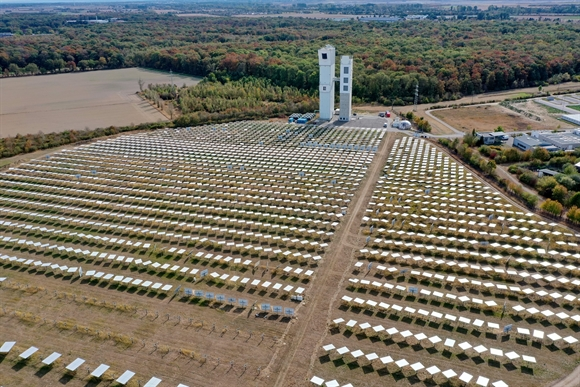
\includegraphics[width=0.7\textwidth]{fig/SolarkraftwerkJuelich.jpg}}
\caption[Solarthermisches Demonstrations- und Versuchskraftwerk Jülich]{Solarthermisches Demonstrations- und Versuchskraftwerk Jülich \cite{DLRSolartürmeBild}}
    \label{fig_Solarturm}
\end{figure}

Die solare Strahlung wird durch gezielte Ausrichtung der Heliostaten auf die Spitze des Solarturms, an der sich der Receiver befindet, konzentriert.
Dieser absorbiert die Strahlung, und gibt sie an ein Wärmeträgermedium ab, welches dann dem sich anschließenden Prozess zur Verfügung steht.
Alternativ kann das erhitzte Medium auch zur späteren Verwendung in einem Energiespeicher zwischengespeichert werden \cite[S.11]{DissBelhomme}.
Die schematische Darstellung eines Solarturmkraftwerkes zeigt Abbildung \ref{fig_SchemaSolarturmkraftwerk}, der in dieser Arbeit fokussierte Teil ist hervorgehoben.

\begin{figure}[h!]
    \centering
\setlength{\fboxsep}{5pt}
    \setlength{\fboxrule}{1pt}
\fbox{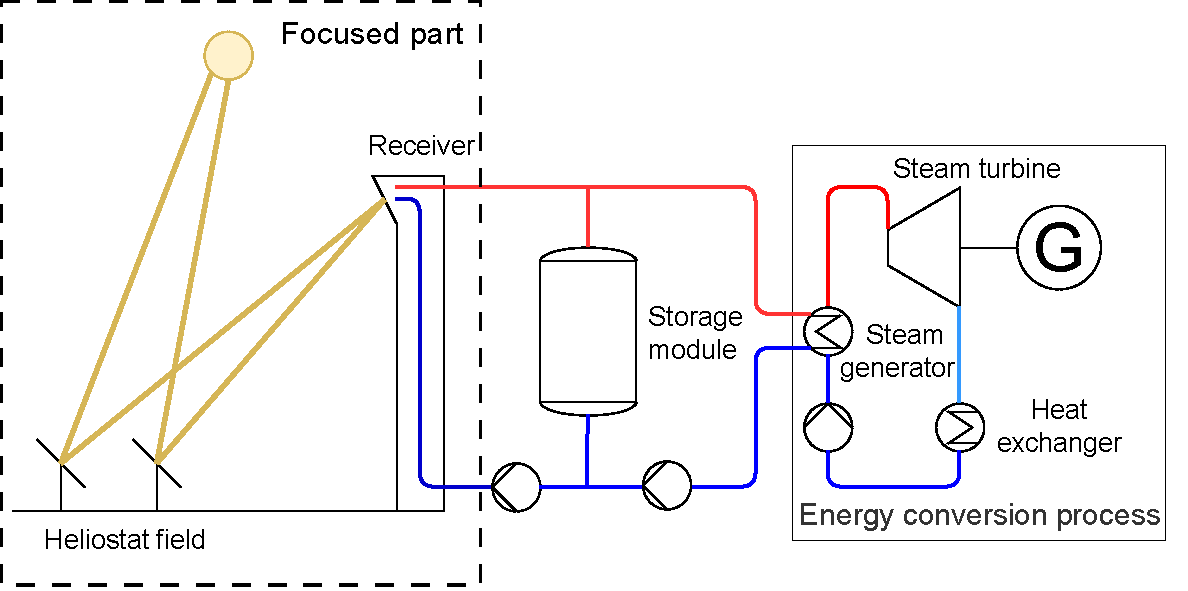
\includegraphics[width=0.9\textwidth]{fig/solar_tower_plant-Page-1.pdf}}
\caption[Vereinfachte schematische Darstellung eines Solarturmkraftwerkes]{Vereinfachte schematische Darstellung eines Solarturmkraftwerkes \cite[S.5]{DissZanger}}
    \label{fig_SchemaSolarturmkraftwerk}
\end{figure}


Der Wärmespeicher und der Energieumwandlungsprozess werden in dieser Arbeit nicht weiter betrachtet.
Im Gegensatz dazu sind die Heliostaten sowie der Receiver und der Einfluss der Sonneneinstrahlung auf diese Komponenten für das weitere Verständnis der Arbeit relevant und werden näher erläutert.


\subsection{Heliostaten} \label{subsec_Heliostaten}
Die Heliostaten sind bidirektional bewegliche Spiegel, die die Sonneneinstrahlung auf den Receiver bündeln.
Jeder Heliostat besteht aus einer reflektierenden Fläche, einer tragenden Struktur und einem Nachführmechanismus.
Letzterer ist erforderlich, um den Brennfleck auch bei wechselnden Sonnenständen statisch zu halten.
Dafür verstellt eine integrierte Steuereinheit auf Basis des Sonnenstandes die reflektierende Fläche entsprechend.
Die beiden Freiheitsgrade der Heliostaten sind die Drehung in der Elevations- und der Azimut-Ebene, wie sie in Abbildung \ref{fig_FreiheitsgradeHeliostat} dargestellt sind. \cite[S.13]{DissBelhomme}

\begin{figure}[h!]
    \centering
    \setlength{\fboxsep}{1pt}
    \setlength{\fboxrule}{1pt}
    \fbox{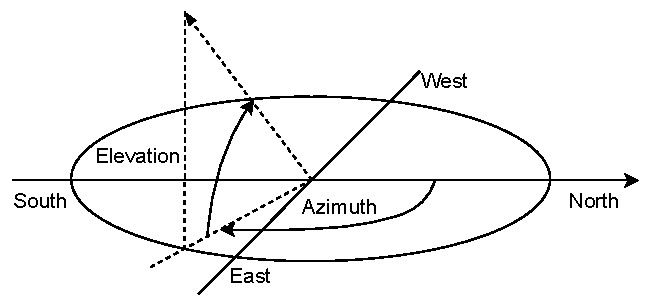
\includegraphics[width=0.7\textwidth]{fig/FreiheitsgradeHeliostat.pdf}}
\caption[Darstellung der Elevations- und Azimut-Ebene]{Darstellung der Elevations- und Azimut-Ebene \cite[S.6]{DissZanger}}
    \label{fig_FreiheitsgradeHeliostat}
\end{figure}

Größe, Form und Art der spiegelnden Fläche unterscheiden sich bei verschiedenen Heliostat-Typen.
Die Spiegelfläche ist zwar bei allen Heliostaten in der Regel rechteckig, besteht bei größeren Heliostaten jedoch aus mehreren kleinen Spiegeln, sog. \textit{Facetten}.
Um eine geforderte Brennweite erreichen zu können, sind diese Facetten in einer Ebene oder zueinander gekippt angeordnet.
Eine Krümmung der Fläche nach innen erzielt eine höhere Konzentration der Strahlung. \cite[S.5]{DissZanger}

Der tragende Körper bei Heliostaten jeder Größe normalerweise aus wirtschaftlichen Gründen aus einer T-Struktur \cite[S.97]{ScottAJones}.
Im Gegensatz zu den bei großen Heliostaten zur Nachführung eingesetzten Schneckengetriebeeinheiten, kommen bei Kleinheliostaten Schubstangenmotoren zum Einsatz.
Die Heliostaten am Betrachtungsstandort Jülich bestehen aus vier ebenen, rechteckigen Facetten auf einem T-Träger und sind mit einer Reflexionsfläche von $\SI{8.3}{\metre\squared}$ vergleichsweise klein \cite[S.4]{DissGall}\cite[S.13]{DissBelhomme}.
Auf der \textit{PS10} (Planta Solar 10) bei Sevilla stehen beispielsweise Heliostaten mit $\SI{120}{\metre\squared}$ Reflexionsfläche aufgeteilt auf 28 Facetten \cite[S.5]{ManuelSilva}.
Die nachfolgende Abbildung \ref{fig_DarstellungHeliostat} soll die grundsätzliche Ähnlichkeit im Aufbau der Heliostaten auch bei unterschiedlicher Größe zeigen.

\begin{figure}[h!]
    \centering
    \setlength{\fboxsep}{1pt}
    \setlength{\fboxrule}{1pt}
    \fbox{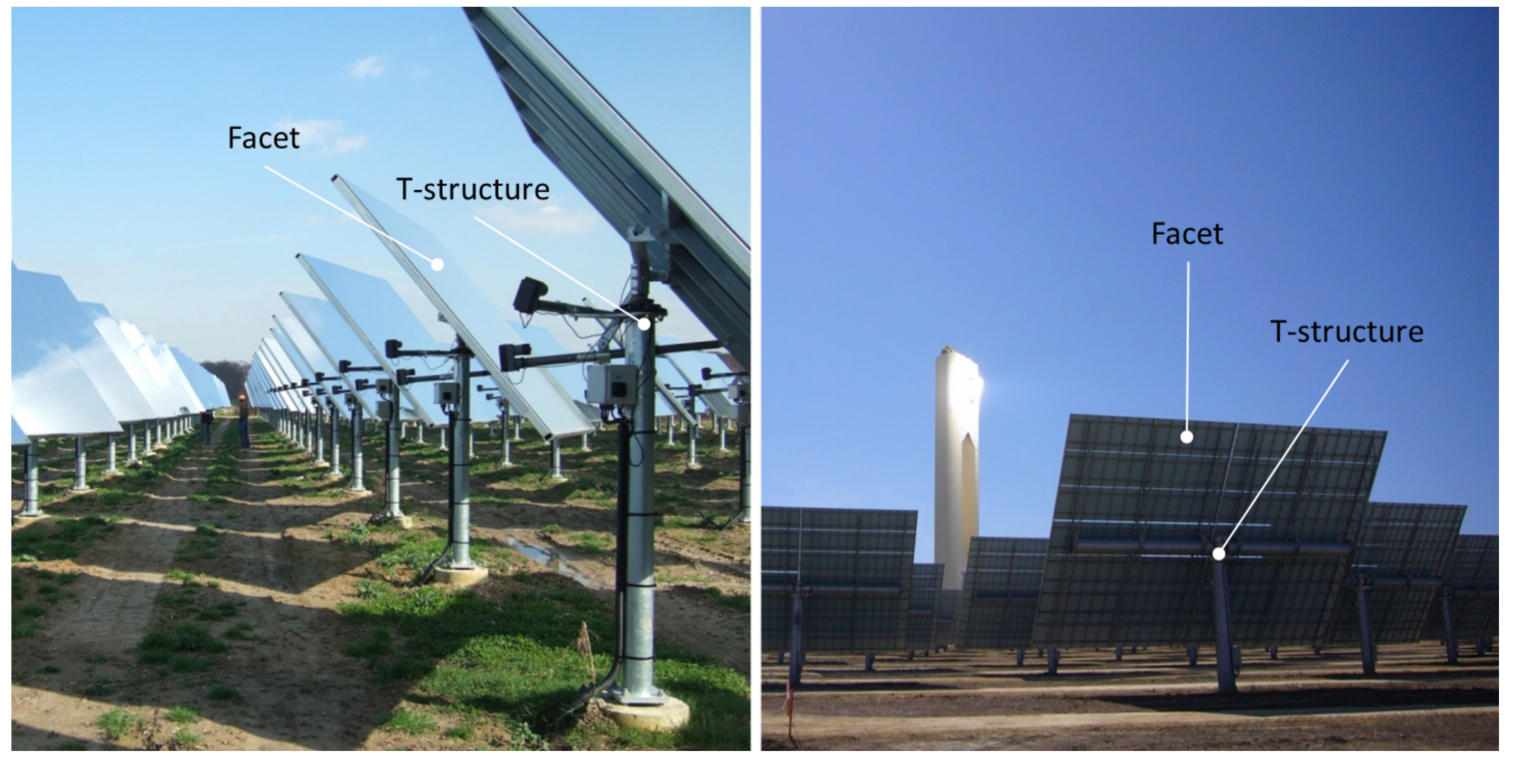
\includegraphics[width=1\textwidth]{fig/Heliostat.png}}
\caption[Ausra Heliostat am Forschungsstandort Jülich mit $\SI{8.3}{\metre\squared}$  und Sanlúcar-120-Heliostat auf der PS10 bei Sevilla mit $\SI{120}{\metre\squared}$ Reflexionsfläche]{Ausra Heliostat am Forschungsstandort Jülich mit $\SI{8.3}{\metre\squared}$  (links) und Sanlúcar-120-Heliostat auf der PS10 bei Sevilla mit $\SI{120}{\metre\squared}$ Reflexionsfläche (rechts) \cite[S.13]{DissBelhomme}}
    \label{fig_DarstellungHeliostat}
\end{figure}

Die Gesamtheit der Heliostaten, die um den Receiver eines Solarturms angeordnet sind, wird als Heliostatenfeld bezeichnet.
Dieses besteht normalerweise aus identischen Heliostaten, welche in Reihen oder konzentrischen Kreisen angeordnet sind.
Denkbare Anordnungen sind Rundum-, Nord- und Südfelder (siehe Abbildung \ref{fig_AnordnungHeliostatfeld}); die effizienteste Anordnung ist besonders von der geografischen Lage abhängig.
Effektiv sind Solarturmkraftwerke vor allem bei steilen Einfallswinkeln der Sonne auf die Spiegel (vgl. Kapitel \ref{subsubsec_KosinusVerluste}).
Damit ergibt sich zwangsläufig, dass in Polnähe einseitige Felder  eine höhere Feldausbeute erreichen während in Äquatornähe Rundum-Felder effektiver sind.
Wie in Abbildung \ref{fig_Solarturm} zu sehen ist, handelt es sich in Jülich um ein einseitiges, nach Norden ausgerichtetes Feld, bestehend aus 2153 Heliostaten.

\begin{figure}[h!]
    \centering
    \setlength{\fboxsep}{1pt}
    \setlength{\fboxrule}{1pt}
    \fbox{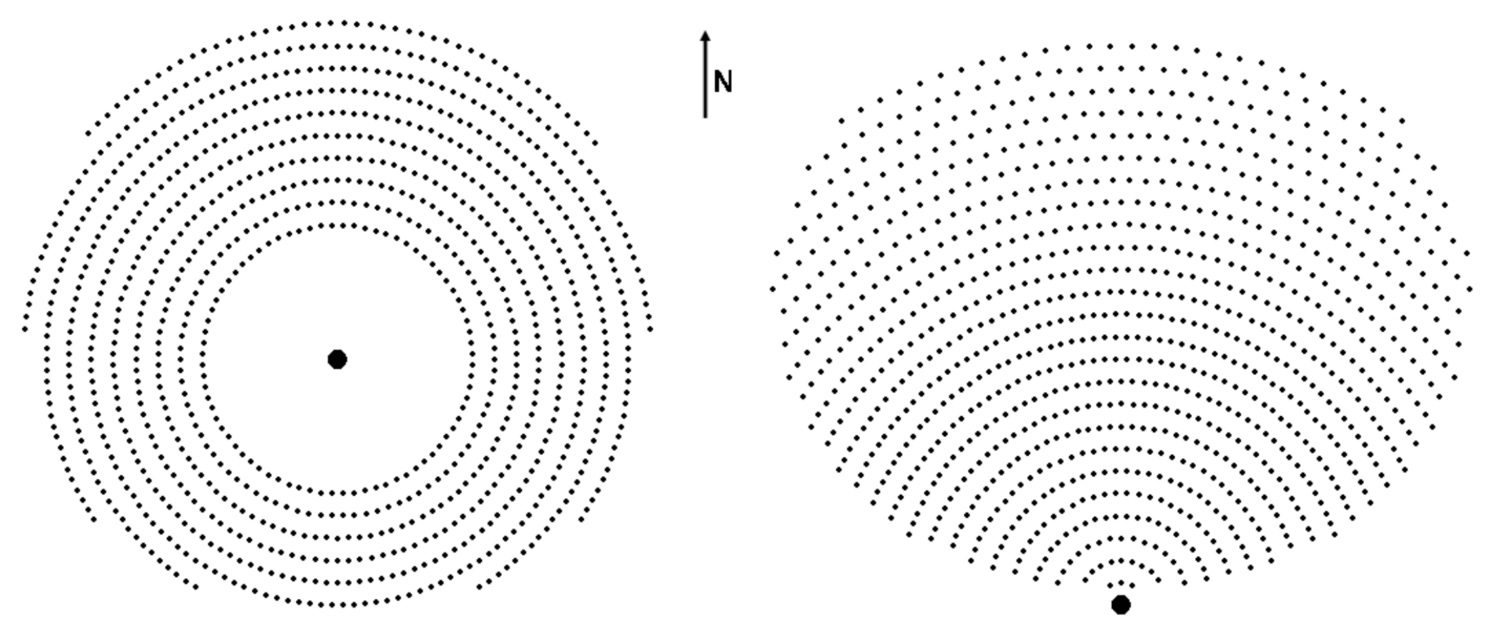
\includegraphics[width=1\textwidth]{fig/Vergleich_Heliostatenfelder.png}}
\caption[Verschiedene Heliostatfeld-Layouts auf der Nordhalbkugel: Rundum-Feld und Nordfeld]{Verschiedene Heliostatfeld-Layouts auf der Nordhalbkugel: Rundum-Feld (links) und Nordfeld (rechts) \cite[S.14]{DissBelhomme}}
    \label{fig_AnordnungHeliostatfeld}
\end{figure}

\subsection{Receiver} \label{subsec_Receiver}

Die Aufgabe des Receivers ist die Absorption der reflektierten Sonneneinstrahlung.
Durch Konvektion wird die absorbierte Energie an ein Wärmeträgermedium weitergegeben, das zur weiteren Verwertung oder Speicherung zur Verfügung steht.
Receiver von Solarturmkraftwerken unterscheiden sich in ihrem Aufbau, Wärmeträgermedium, Material und den damit einhergehenden physikalischen Grenzen.

Grundsätzlich muss zwischen zylindrischen und rechteckigen Receivern unterschieden werden.
Erstere kommen bei Rundum-Feldern zum Einsatz, letztere bei Nord- oder Südfeldern.
Je nach Standort und Anwendungsfall kommen sog. \textit{Cavity}-Receiver zum Einsatz, welche nach innen gebogen sind um vor Wärmeverlust durch zu schnelle Windgeschwindigkeiten an der Receiver Vorderseite zu schützen. \cite{Flesch}

Das Material des Receivers ist abhängig vom genutzten Wärmeträgermedium.
Typische Medien sind Luft, geschmolzene Salze oder Wasser.
Für Wasser oder Salzschmelzen werden meist Receiver aus Metallrohren unterschiedlicher Hochtemperatur-Legierungen verwendet.
Für Receiver mit Luft als Wärmeüberträgermedium, wie beispielsweise in Jülich, wird zumeist eine poröse Keramik genutzt. \cite{Barlev}\cite{Ho2017}

Wenn Eigenschaften wie die maximal zulässigen thermischen Spannungen des Receivers überschritten werden, kann dieser beschädigt werden \cite{AlbertoSanchez}.
Bei einem Receiver mit Salzschmelze als Medium hängt diese beispielsweise mit der lokalen Salztemperatur und -geschwindigkeit sowie der Windgeschwindigkeit zusammen \cite{VantHull}.
Dabei wird die lokale Salztemperatur direkt durch die solare Einstrahlung auf dem Receiver beeinflusst.

Eine Möglichkeit, die Einhaltung der maximalen thermischen Spannungen zu gewährleisten, ist also unter anderem die Einführung einer maximalen Flussdichte am Receiver, die auf der Grundlage seiner spezifischen Eigenschaften berechnet werden kann.
Dabei ist der zulässige Wert auch stark vom verwendeten Wärmeträgermedium abhängig.
Für Rohrreceiver, die mit flüssigem Natrium gekühlt werden, sind beispielsweise maximale Strahlungsflussdichten von $\SI{2.5}{\mega\watt\per\square\metre}$ erlaubt, während bei luftgekühlten Rohrreceivern nur $\SI{200}{\kilo\watt\per\square\meter}$ \cite[S.17]{DissBelhomme} erreicht werden dürfen.

Die Flussdichte $\phi$ ist dabei als Strahlungsfluss $F$ pro Fläche $A$ zu verstehen, wobei $F$ das Verhältnis aus absorbierter Strahlungsenergie $Q$ pro Zeiteinheit $t$ darstellt (siehe Formel \ref{eq_Strahlungsfluss} und \ref{eq_Flussdichte}).

\begin{equation} \label{eq_Strahlungsfluss}
    F = \frac{\text{d}Q}{\text{d} t}
\end{equation}
% \centerline{\small{\textsf{\textbf{Formel \ref{eq_Strahlungsfluss}:}} Berechnung des Strahlungsflusses $F$}}
\myequations{\quad Berechnung des Strahlungsflusses $F$}
\vspace*{-\baselineskip}
\begin{equation} \label{eq_Flussdichte}
    \phi = \frac{\text{d}F}{\text{d} A}
\end{equation}
% \centerline{\small{\textsf{\textbf{Formel \ref{eq_Flussdichte}:}} Berechnung der Flussdichte $\phi$}}
\myequations{\quad Berechnung der Flussdichte $\phi$}

Zur Bestimmung der Leistung, die dem System auf diese Weise zugeführt wird, kann die Flussdichte verwendet werden.
Sie ergibt sich aus der Integration der Flussdichte $\phi$ über der Fläche des Receivers.

\begin{equation} \label{eq_LeistungReceiver}
    P = \int_{A}\phi~\text{d} A
\end{equation}
% \centerline{\small{\textsf{\textbf{Formel \ref{eq_LeistungReceiver}:}} Berechnung Bruttoleistung $P$ auf dem Receiver}}
\myequations{\quad Berechnung Leistung $P$ auf dem Receiver}

Je nach Anwendungsfall kann auch ein Limit für die minimal erlaubte Flussdichte auf dem Receiver existieren, um beispielsweise das Problem von Verfestigung von Salzschmelzen zu vermeiden.
Da das in dieser Arbeit untersuchte Turmkraftwerk in Jülich jedoch mit einem ebenen, rechteckigen Receiver aus Keramik und mit Luft als Medium ausgestattet ist, wird dies hier nicht weiter betrachtet.

\subsection{Optische Verluste} \label{subsec_OptischeVerluste}
Um den effizientesten Betrieb solarer Turmkraftwerke zu erreichen, ist die Minimierung optischer Verluste wesentlich.
Diese optischen Verluste sind einerseits geografischer Natur, aber auch durch die Wirkweise der Heliostaten bedingt und werden nachfolgend erläutert.
Auf meteorologische Einflüsse wird in Kapitel \ref{sec_Nowcasting} näher eingegangen.

\subsubsection*{Kosinus-Verluste} \label{subsubsec_KosinusVerluste}
Die \textit{Kosinus-Verluste} sind ein geografischer Einflussfaktor.
Die Sonnenstrahlen (\textit{solar radiation}) treffen auf die Spiegeloberfläche (\textit{mirror}) unter einem bestimmten Winkel, der von Sonnenstand und Ausrichtung des Spiegels abhängt.
Dieser Winkel bestimmt die effektive Reflexionsfläche (\textit{effective refelction surface}), welche senkrecht zur Einfallsrichtung der Strahlung projiziert wird.
Wie in Abbildung \ref{fig_KosinusVerlust} zu erkennen ist, entspricht das Verhältnis zwischen der effektiven Fläche und der Gesamtfläche jedes Heliostaten dem Kosinus des Winkels zwischen der Einfallsrichtung und der Hauptnormalen der Spiegelfläche (\textit{main normal}).
Bei zunehmendem Winkel $\beta$, also ungünstigeren Lichteinfallswinkeln, nimmt die effektive Fläche ab und die Effizienz der Heliostaten wird geringer.
Diese wird mit dem Kosinus-Wirkungsgrad $\cos\beta$ ausgedrückt, der also in direktem Zusammenhang mit der reflektierten Sonnenleistung steht.
Der Einfluss der Kosinus-Verluste zeigt sich beispielsweise an Untersuchungen am Solar One Tower in Süd-Kalifornien, dort schwankt der Kosinus-Wirkungsgrad in dieser Gegend\linebreak jährlich zwischen $\SI{0.65}{}$ und $\SI{0.9}{}$, je nach Sonnenstand und damit verbundener Heliostatenposition. \cite{Holl}

\begin{figure}[h!]
    \centering
    \setlength{\fboxsep}{1pt}
    \setlength{\fboxrule}{1pt}
    \fbox{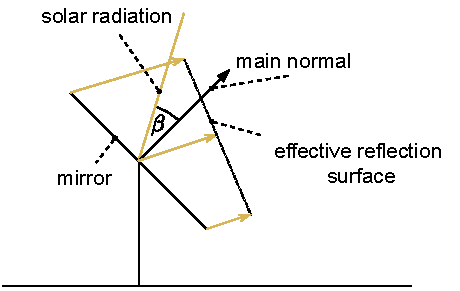
\includegraphics[width=0.6\textwidth]{fig/KosinusVerluste}}
\caption[Seitenansicht eines Heliostaten zur Verdeutlichung des Winkels $\beta$ im Kontext der Kosinus-Verluste]{Seitenansicht eines Heliostaten zur Verdeutlichung des Winkels $\beta$ im Kontext der Kosinus-Verluste \cite[S.7]{DissZanger}}
    \label{fig_KosinusVerlust}
\end{figure}


\subsubsection*{Reflexionsverluste} \label{subsubsec_Reflexionsverluste}
Wenn das Sonnenlicht auf die Spiegel trifft, wird ein Teil absorbiert, was die Menge des reflektierten Lichts verringert.
Diese Verringerung des Reflexionsvermögens wird durch Umweltfaktoren wie Regen und Staub weiter verstärkt.
Reflektieren saubere Spiegeloberflächen normalerweise zwischen $\SIrange{87}{94}{\percent}$ des auf sie treffenden Sonnenlichts, sinkt dieser Wert durch umweltbedingte Verschmutzung bis auf $\SI{80}{\percent}$. \cite[S.14]{DissBelhomme}

\subsubsection*{Blockierung und Abschattung} \label{subsubsec_blockingshading}
Je nach Sonnenstand, Heliostatanordnung und Objekten mit Schattenwurf, wie dem Turm, werden Heliostaten verschattet oder \gans{blockiert}.
Im Falle einer \textit{Abschattung} ist der direkte Weg zwischen Sonne und Heliostat (teilweise) versperrt, sodass die Sonnenstrahlung nicht ungehindert auf die Spiegelfläche treffen kann.
Bei der \textit{Blockierung} ist der Weg zwischen Heliostat und Receiver betroffen; die reflektierte Strahlung eines Heliostaten wird durch einen anderen Heliostaten (teilweise) blockiert.
Abbildung \ref{fig_AbschattungBlockieren} visualisiert dies.
Das Problem der Abschattung betrifft alle Heliostaten und tritt besonders bei niedrigen Sonnenständen auf.
Im Gegensatz dazu sind von der Blockierung, unabhängig vom Sonnenstand, zumeist die hinteren Heliostatenreihen betroffen.
Durch ein geeignetes Felddesign kann diesen Verlusten entgegengewirkt werden. \cite[S.686]{Wei2010}

\begin{figure}[h!]
    \centering
    \setlength{\fboxsep}{1pt}
    \setlength{\fboxrule}{1pt}
    \fbox{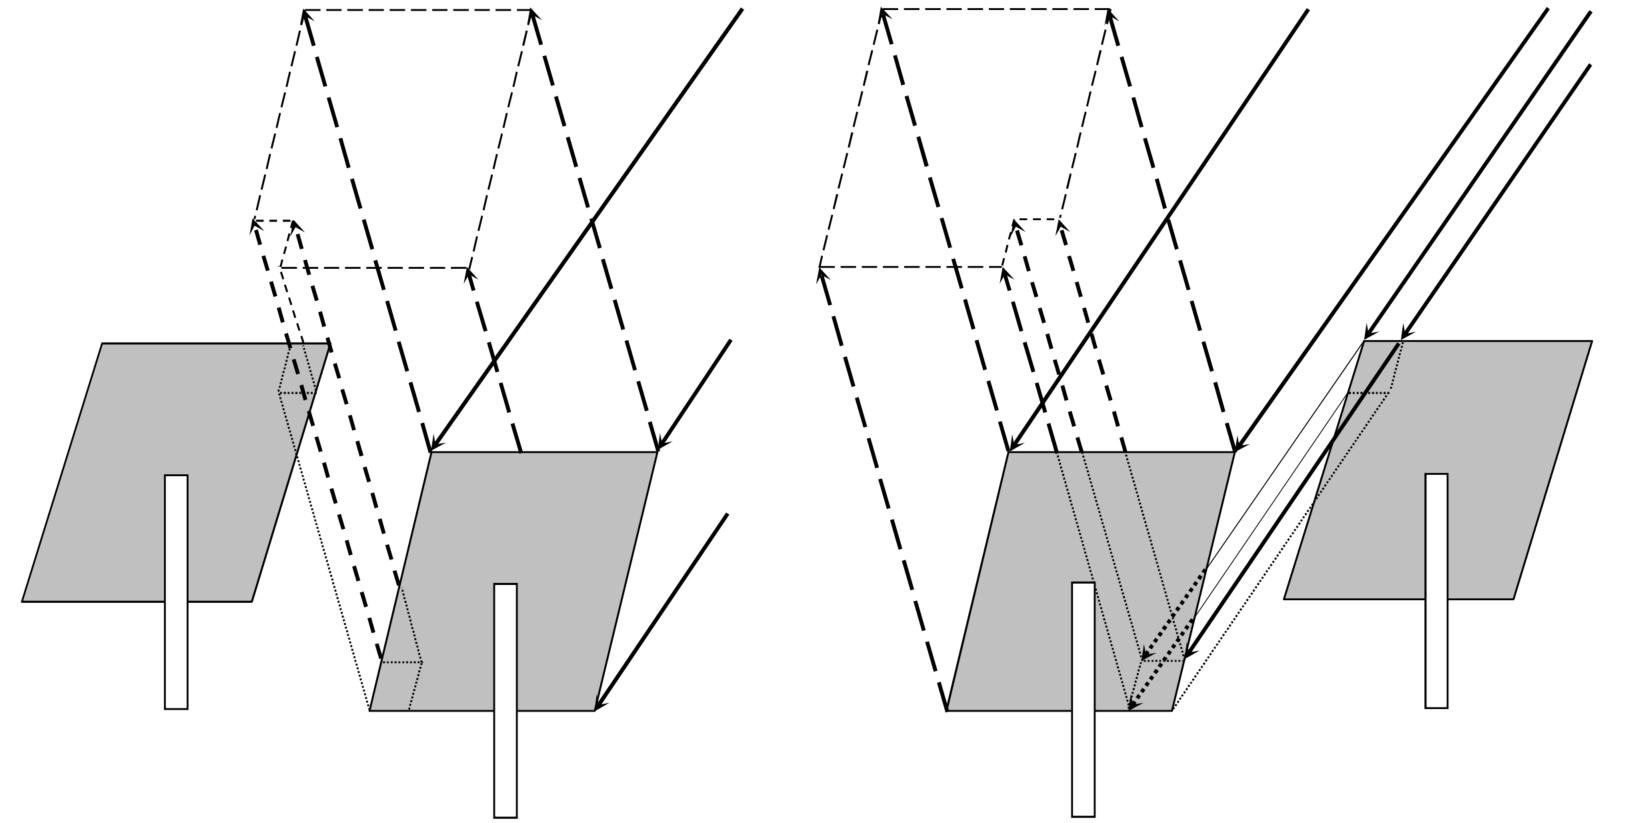
\includegraphics[width=1\textwidth]{fig/BlockingShading.png}}
\caption[Blockierung und Abschattung von Heliostaten]{Blockierung (links) und Abschattung (rechts) von Heliostaten \cite[S.15]{DissBelhomme}}
    \label{fig_AbschattungBlockieren}
\end{figure}

\subsubsection*{Spiegelfehler} \label{subsubsec_Spiegelfehler}
Ein weiterer optischer Verlustfaktor sind die \textit{Spiegelfehler}.
Als solche werden Abweichungen eines Spiegels von seiner idealen Form genannt, welche den Spiegel wellig erscheinen lassen.
Hervorgerufen wird dieser Fehler beispielsweise durch innere Spannungen in der Heliostatenstruktur als Folge von Wind oder Temperaturschwankungen oder aber durch Ungenauigkeiten in der Herstellung.
Die Größe des Fehlers wird als Winkel zwischen dem tatsächlichen Normalvektor des Spiegels und dem idealen Normalvektor gemessen und liegt in der Regel zwischen $\SI{1.5}{\milli\radian}$ und $\SI{2.5}{\milli\radian}$. \cite[S.16]{DissBelhomme}

\subsubsection*{Streuung} \label{subsubsec_Streuung}
Als \textit{Streuung} bezeichnet man den Teil der reflektierten Sonnenstrahlung, der den Receiver verfehlt und nicht in nutzbare Energie umgewandelt werden kann.
Dies geschieht beispielsweise durch die oben genannten Spiegelfehler oder wenn der Abstand zwischen Heliostat und Receiver so groß ist, dass das Abbild der Reflexion auf dem Receiver größer ist als der Receiver selbst. \cite[S.15-16]{DissBelhomme}

\subsubsection*{Nachführfehler} \label{subsubsec_Nachführfehler}
Der Nachführfehler beschreibt die fehlerhafte Ausrichtung der Heliostaten.
Er kann durch Schmutz oder Verschleiß an den Nachführachsen, oder Ungenauigkeiten bei der Motorausrichtung und Sonnenstandsmessung hervorgerufen werden \cite[S.7]{Richter}. Auch dieser Fehler wird als Winkel gemessen und liegt normalerweise bei $\SI{0.5}{\milli\radian}$ bis $\SI{2}{\milli\radian}$ \cite[S.17]{DissBelhomme}.

\subsubsection*{Atmosphärische Abschwächung} \label{subsubsec_AtmosphärischeAbschwächung}
Die reflektierte Strahlung wird auf dem Weg zwischen Heliostat und Receiver durch Absorption und Streuung an Luftmolekülen abgeschwächt.
Die Intensität der Abschwächung ist von der Höhe des Heliostatenfeldes über dem Meeresspiegel und der lokalen Luftfeuchtigkeit, besonders aber von der Distanz zwischen Heliostat und Receiver, abhängig.
Bei einem Abstand von $\SI{1000}{\metre}$ kann dir Abschwächung bis zu $\SI{1.2}{\percent}$ betragen \cite[S.121]{Biggs}\cite[S.17]{DissBelhomme}.



\section{Nowcasting-Systeme zur Wettervorhersage} \label{sec_Nowcasting}
Ein wesentlicher Schwerpunkt dieser Arbeit liegt in der Analyse des Wolkeneinflusses, welcher als meteorologischer optischen Verlust auf das Gesamtsystem des Solarturms einwirkt.
Um eine zuverlässige Regelung hinsichtlich der im Kapitel \ref{subsec_Receiver} beschriebenen physikalischen Grenzen des Receivermaterials zu gewährleisten, ist eine möglichst genaue Wolkenvorhersage unerlässlich.
In der Praxis wird dies durch die sogenannten \textit{Nowcasting Systeme} erreicht, die im Gegensatz zu den klassischen Modellen der Wettervorhersage durch zeitlich und räumlich hochauflösende Beobachtungen genauere lokale Vorhersagen liefern \cite{DWD1}.

Für deutschlandweit flächendeckende Vorhersagen nutzt der deutsche Wetterdienst u.~a. Sensorik zur Überwachung von Luftdruck, -temperatur und -feuchte sowie Radarsysteme und Satellitenbilder \cite{DWD1}\cite{DWD0}.
Durch Abruf und Verarbeitung dieser Daten im 5-Minutentakt können regionale Wetterprognosen für die kommenden Stunden generiert werden.

Für den Anwendungsfall des Solarturms ist eine solche Prognose jedoch nicht ausreichend.
Je präziser die jeweils lokale Vorhersage für das Heliostatenfeld ist, desto effektiver ist die Regelung.
Da die Auflösung der deutschlandweiten Vorhersage lediglich rund $\SI{1}{\kilo\metre} \times \SI{1}{\kilo\metre}$\linebreak beträgt \cite{DWD1}\cite{DWD2}, während sich das Heliostatenfeld in Jülch auf eine Fläche von rund\linebreak $\SI{330}{\metre} \times \SI{310}{\metre}$ beschränkt, sind lediglich sehr grobe Vorhersagen zu erwarten.
Darüber hinaus ist auch die zeitliche Auflösung von 5 Minuten \cite{DWD2} unterhalb der Möglichkeiten anderer Nowcasting Systeme \cite{DLRNowcasting}\cite[S.272]{QuesadaRuiz}.

Ein Instrument für zeitlich und räumlich hochauflösende Vorhersagen sind die sogenannten \gans{All-sky imagers} (\textit{ASI}) in Kombination mit Pyrheliometern.
Bei ASIs handelt es sich um nach oben gerichtete Kameras, welche $\SI{180}{\degree} \times \SI{180}{\degree}$ halbkugelförmige Bilder mit dem Zweck der Wolkenüberwachung erzeugen.
Pyrheliometer sind Messgeräte zur Ermittlung der direkten Sonneneinstrahlung (der \textit{direct normal irradiation}, kurz: \textit{DNI}).
Der Prozess zur Erstellung von Nowcasting Vorhersagen auf Basis dieser Bilder und Messdaten wird beispielsweise von Samu \textit{et al.} in \cite{Samu} beschrieben.

Das DLR verwendet in Spanien und Jülich bereits ein Nowcasting System auf Basis der ASIs.
Es erstellt in subminütlicher Auflösung Einstrahlungskarten des betrachteten Solarfeldes mit einer räumlichen Auflösung von bis zu $\SI{20}{\metre} \times \SI{20}{\metre}$.
Tabelle \ref{tab_VorgehenNowcasting} fasst alle Schritte zur Erstellung dieser Karten zusammen. \cite[S.4,S.13]{Samu}\cite{DLRNowcasting}.

\begingroup
\renewcommand{\arraystretch}{1.2}
\begin{table}[ht!]
    \caption[Vorgehen zur Erstellung der Einstrahlungskarten im Nowcasting mittels ASIs]{Vorgehen zur Erstellung der Einstrahlungskarten im Nowcasting mittels ASIs (nach\cite[S.4]{Samu})}
    \centering
    \begin{tabular}{m{0.1\textwidth}m{0.85\textwidth}}
        \rowcolor{white}
\toprule
        Schritt & Beschreibung                                   \\
        \midrule
        1       & Wolkensegmentierung                            \\
        2       & Bestimmung der 3D Koordinaten der Wolken       \\
        3       & Extraktion der Wolkenbewegung                  \\
        4       & Vorhersage der zukünftigen Wolkenpositionen    \\
        5       & Ermittlung der Lichtdurchlässigkeit der Wolken \\
        6       & Errechnen des Schattenwurfs                    \\
        7       & Erstellung der Einstrahlungskarten             \\
\toprule
    \end{tabular}
    \label{tab_VorgehenNowcasting}
\end{table}
\endgroup

Im Rahmen der Segmentierung (Schritt 1) wird durch Bilderkennung (z.~B. mittels neuronaler Netzwerke) festgestellt, welche der aufgenommenen Pixel zu Wolken gehören.
Für die Bestimmung der Wolkenpositionen (2) werden mindestens zwei ASIs benötigt, welche den Himmel zeitgleich aus unterschiedlichen Winkeln aufnehmen.
Zu diesem Zweck werden sie rund $\SIrange{500}{1000}{\metre}$ entfernt voneinander positioniert.
Der Effekt der Stereoskopie ermöglicht auf dieser Basis die Bestimmung der Position und Ausdehnung im dreidimensionalen Raum \cite[S.5]{Samu}.
Durch Analyse aufeinander folgender Bilder der Kameras kann die jeweilige Wolkenbewegung erfasst werden (3), die Aufschluss über die zukünftigen Positionen dieser Wolken (4) gibt.
Die nachfolgende Abbildung \ref{fig_Nowcasting} visualisiert exemplarisch, den jeweiligen Informationsgehalt der unbearbeiteten Kamerabilder (Links), der Bilder nach Segmentierung (Mitte) und nach Extraktion der Bewegungsvektoren (Rechts).

\begin{figure}[h!]
\centering
\setlength{\fboxsep}{1pt}
\setlength{\fboxrule}{1pt}
\fbox{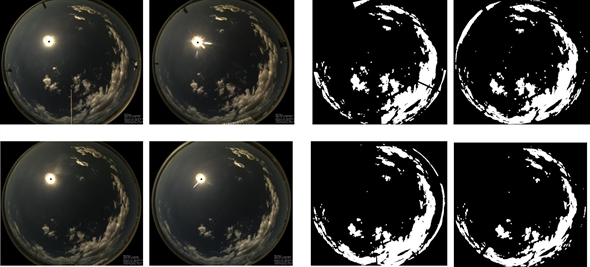
\includegraphics[width=1\textwidth]{fig/Nowcasting}}
\caption[Beispiel eines unbearbeiteten ASI-Bildes, eines segmentierten Bildes und eines Bildes inklusive visualisierter Bewegungsvektoren]{Beispiel eines unbearbeiteten ASI-Bildes (Links), eines segmentierten Bildes (Mitte) und eines Bildes inklusive visualisierter Bewegungsvektoren (Rechts) (nach \cite[S.8]{Sayeef})}
\label{fig_Nowcasting}
\end{figure}

Die Ermittlung der Lichtdurchlässigkeit der Wolken (5) geschieht mithilfe der Messwerte von Pyrheliometern.
Sofern die betrachtete Wolke im direkten Weg zwischen Sonne und Pyrheliometer liegt, kann aus den Messwerten direkt die Lichtdurchlässigkeit der Wolke bestimmt werden.
Andernfalls ergibt sich die Durchlässigkeit aus einer Wahrscheinlichkeitsanalyse mit historischen Wolkenhöhen- und Transmissionsmessungen sowie aktuellen Transmissionsmessungen anderer Wolken und deren Wolkenhöhen \cite{BijanNowcasting}.

Durch Erfassung der Sonnenposition aus den Bildern der ASIs sowie der Wolkenpositionen und -bewegungsvektoren kann die resultierende lokale Verschattung geometrisch bestimmt werden (6).
In Kombination mit der Lichtdurchlässigkeit ergeben sich zu dem aktuellen Zeitpunkt sowie prädiktiv in der benötigten zeitlichen Auflösung und über einen Horizont von $\SIrange{15}{60}{\minute}$ die Einstrahlungskarten (7).
Beispielhaft ist dies als Ergebnis des Nowcastings in Abbildung \ref{fig_EinstrahlungNowcasting} zu sehen.
Das insgesamt überwachte Feld erstreckt sich über $\SI{8}{\kilo\metre} \times \SI{8}{\kilo\metre}$, jedes einzelne Pixel stellt den Einstrahlungswert für eine Fläche von $\SI{20}{\metre} \times \SI{20}{\metre}$ dar. \cite[S.14]{Samu}

\enlargethispage{\baselineskip}
\begin{figure}[h!]
    \centering
    \setlength{\fboxsep}{1pt}
    \setlength{\fboxrule}{1pt}
\fbox{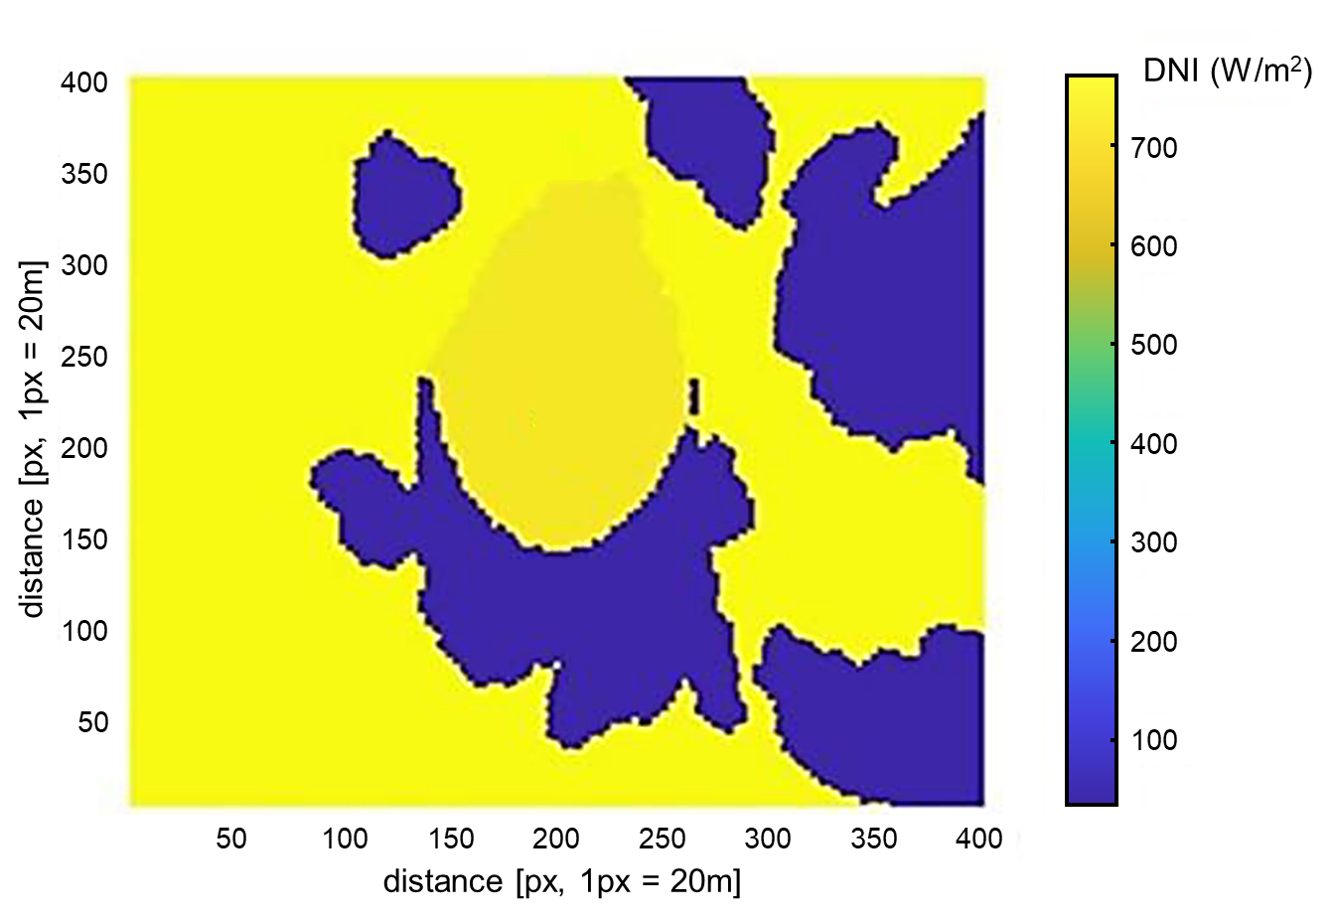
\includegraphics[width=0.77\textwidth]{fig/NowcastingDNIMap}}
    \caption[Beispielhafte Darstellung der Einstrahlungskarte als Ergebnis des Nowcastings]{Beispielhafte Darstellung der Einstrahlungskarte als Ergebnis des Nowcastings (nach \cite[S.14]{Samu})}
    \label{fig_EinstrahlungNowcasting}
\end{figure}



\section{Modellprädiktive Regelung} \label{sec_ModellprädiktiveRegelung}
Das Ziel eines Reglers ist im Allgemeinen, einen sich zeitlich verändernden Prozess von außen so zu beeinflussen, dass dieser Prozess in einer vorgegebenen Weise abläuft.
Dazu besitzt das zu regelnde System mindestens eine beeinflussbare Größe und eine zurückgeführte Messgröße, die mit einer Führungsgröße verglichen wird.
Weiterhin soll die Wirkung von Störungen so gut wie möglich unterdrückt werden \cite[S.1ff]{Lunze}.
Eine verbreitete Art der Regelung ist die hier vorgestellte modellprädiktive Regelung (kurz \textit{MPR} bzw. \textit{MPC}).

\subsection{Grundlagen} \label{subsec_GrundlagenMPC}
Ein wesentliches Merkmal der MPC ist die Möglichkeit künftige Modellparameter in die Regelung einzubeziehen.
Weiterhin besteht mit MPC die Möglichkeit, komplexe nicht-lineare \mbox{\textit{MIMO}-Systeme} (\textbf{M}ulti \textbf{I}nput \textbf{M}ulti \textbf{O}utput) effektiv zu regeln.
Der wohl bedeutendste Grund dafür, dass MPC in der Praxis mit dem PID-Regler den Stand der Technik ausmacht \cite[S.viii]{Kouvaritakis}, ist jedoch die zusätzliche Möglichkeit, Ein- und Ausgangsgrößen Systems mittels sog. \textit{Constraints} zu limitieren; nachteilig ist jedoch der damit direkt verbundene hohe Rechenaufwand. \cite[S.1-2]{Kouvaritakis}

Der MPC hat diese speziellen Features aufgrund des Zusammenspiels seiner beiden Hauptkomponenten: einer Optimierungseinheit und einem mathematischen Modell des zu regelnden Systems.
Abbildung \ref{fig_RegelkreisMPC} zeigt den Aufbau eines Regelkreises mit dem MPC.
Ein Beispiel für eine zu regelnde Anlage, die (\gans{Plant}), stellt ein Solarturmkraftwerk dar.

\begin{figure}[h!]
    \centering
    \setlength{\fboxsep}{1pt}
    \setlength{\fboxrule}{1pt}
\fbox{\includegraphics[width=0.95\textwidth]{fig/Regelkreis.drawio.pdf}}
\caption[Geschlossener Regelkreis mit einem MPC]{Geschlossener Regelkreis mit einem MPC gemäß\cite[S.2]{Schwenzer}}
    \label{fig_RegelkreisMPC}
\end{figure}

Zum besseren Verständnis des Funktionsprinzips eines modellprädiktiven Reglers dient die nachfolgende Abbildung \ref{fig_MPCVerhalten}.
Es ist erkennbar, dass der Regler zum Zeitpunkt $k$ über die Dauer des gesamten \textit{Prädiktionshorizontes} $N_2$ mittels des hinterlegten Modells die \textit{Ausgangsgröße} $\boldsymbol{y}$ simuliert.
Die Berechnung geschieht dabei in durch die \textit{Sample Time} $T_s$ vorgegebenen Zeitschritten.
Dafür kalkuliert die Optimierungseinheit für den \textit{Regelungshorizont} von Zeitpunkt $k+N_1$ bis $k+N_u$ die optimalen \textit{Stellgrößen} $\boldsymbol{u}$, sodass sich $\boldsymbol{y}$ der \textit{Referenztrajektorie} $\boldsymbol{r}$ so gut wie möglich annähert.
Der Abstand zwischen der Referenztrajektorie und der Ausgangsgröße wird mit dem \textit{Fehler} $\boldsymbol{e}$ bezeichnet, der im Zuge der Regelung minimiert wird.
Nach jedem Zeitschritt $T_s$ wird lediglich die erste kalkulierte Stellgröße an das System weitergegeben, bevor sich die Horizonte um einen Zeitschritt verschieben.
Auf Basis der Rückführung von Messgrößen des Systems ergibt sich das Optimierungsproblem des nächsten \mbox{Zeitschritts. \cite[S.3]{Schwenzer}}

\begin{figure}[h!]
    \centering
    \setlength{\fboxsep}{1pt}
    \setlength{\fboxrule}{1pt}
\fbox{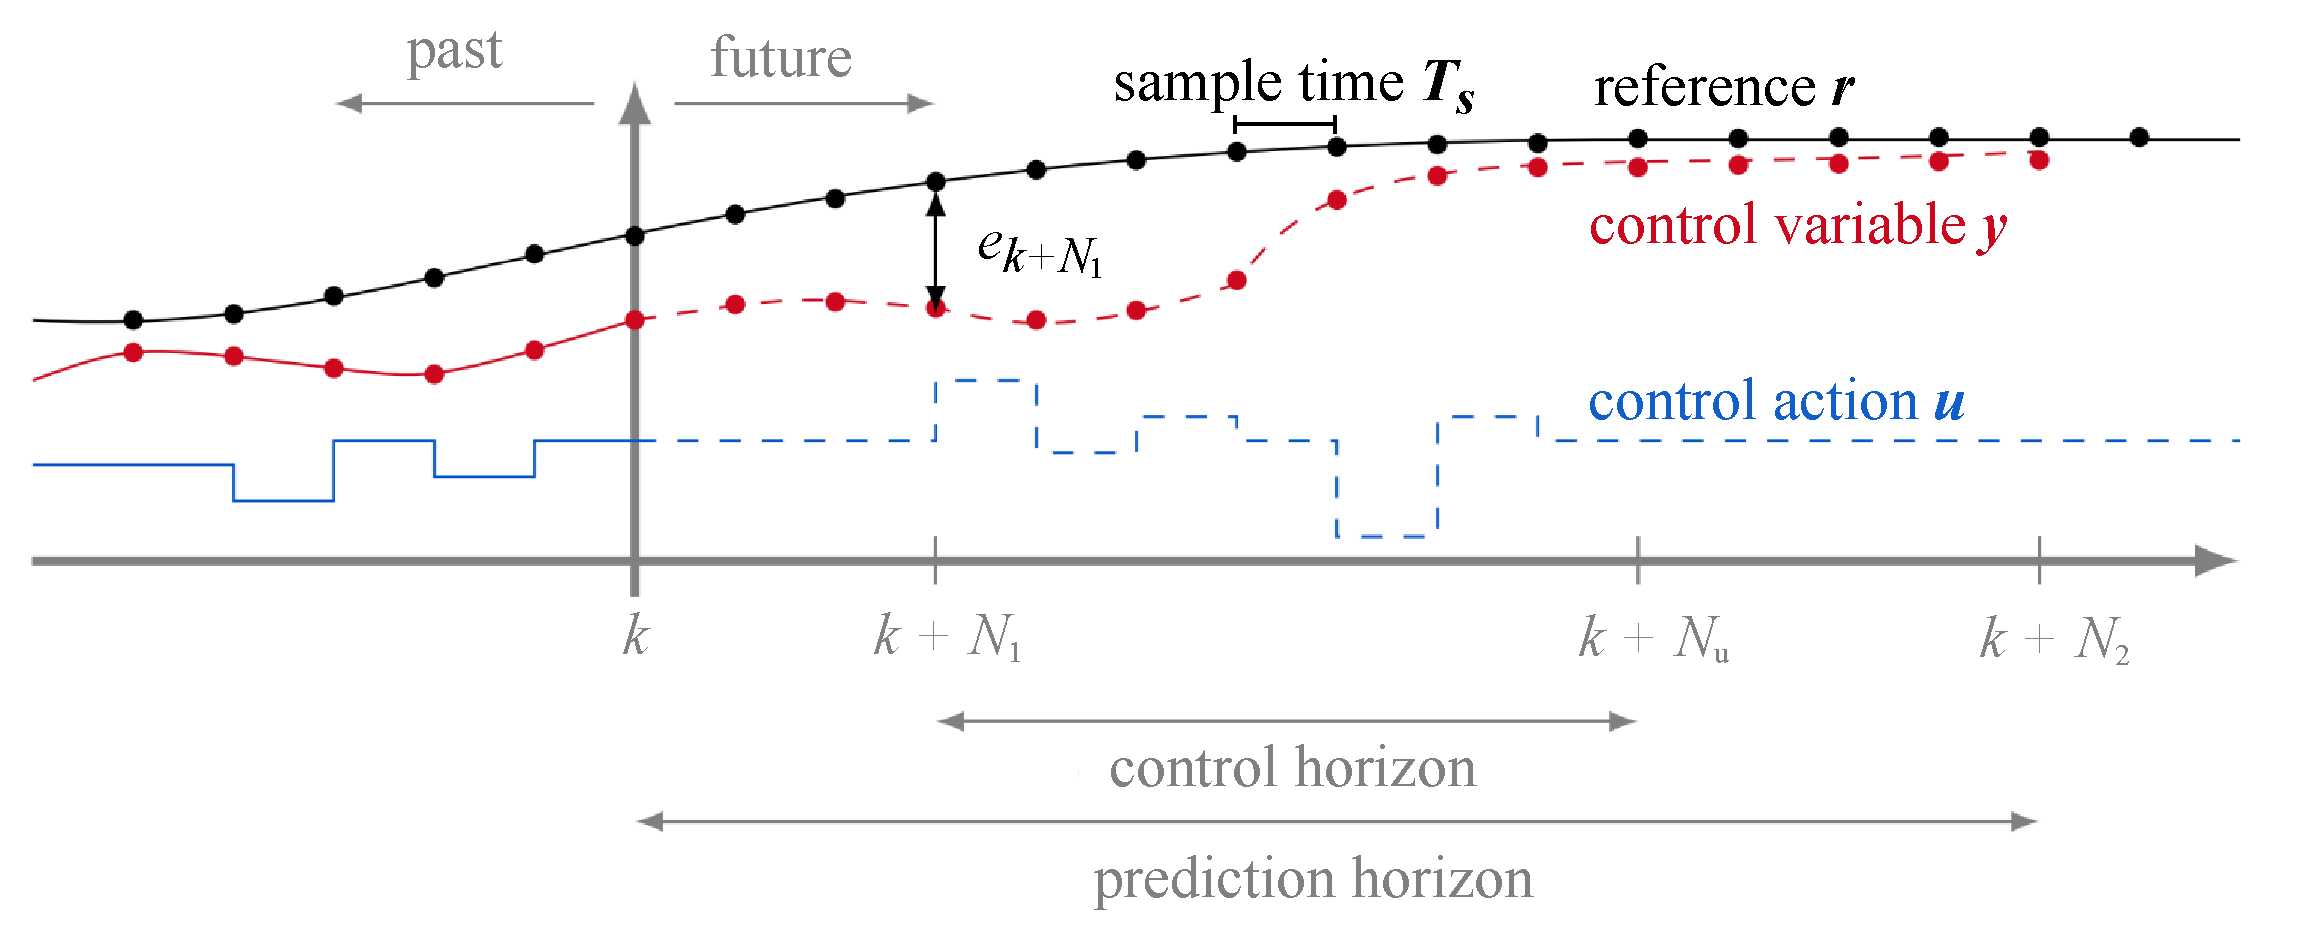
\includegraphics[width=0.95\textwidth]{fig/mpcprinciple}}
\caption[Funktionsprinzip eines MPC]{Funktionsprinzip eines MPC nach \cite[S.3]{Schwenzer} gemäß \cite{Richalet}}
    \label{fig_MPCVerhalten}
\end{figure}

\subsection{Modellierung des Systems} \label{subsec_Modellbildung}
Ein grundlegender Baustein zur erfolgreichen Regelung mit einem modellprädiktiven Regler ist die Abbildung des zu regelnden Systems durch mathematische Formeln – die Modellbildung.
Je präziser das zu regelnde Realmodell in der Modellbildung beschrieben wird, desto genauer werden auch die Ergebnisse der Regelung.
Dabei kann das System sowohl in diskreter als auch kontinuierlicher Form beschrieben werden; für die Optimierung werden kontinuierliche Systeme aus Differenzialgleichungen und algebraischen Gleichungen jedoch in der Regel diskretisiert (vgl. Kapitel \ref{subsec_Diskretisierung}), sodass das System letztlich wie in den Gleichungen \ref{eq_Modellbildung1} - \ref{eq_Modellbildung3} zu beschreiben ist.
Dabei steht $\boldsymbol{x}$ für die dynamischen Modellzustände, $\boldsymbol{u}$ für die Stellgrößen, $\boldsymbol{z}$ für algebraische Größen und $\boldsymbol{p}$ bzw.
$\boldsymbol{p}_{tv}$ für (zeitabhängige, \textbf{t}ime \textbf{v}arying) Modellparameter. \cite[S.3]{Schwenzer}\cite{Dompc1}

\begin{equation} \label{eq_Modellbildung1}
\boldsymbol{x}_{k+1} = f(\boldsymbol{x}_k, \boldsymbol{u}_k, \boldsymbol{z}_k, \boldsymbol{p}_{tv,k}, \boldsymbol{p})
\end{equation}
\myequations{\quad Diskrete Zustandsgleichung in der Modellbildung}
\vspace*{-2.5\baselineskip}
\begin{equation} \label{eq_Modellbildung2}
\mathbf{0} = g(\boldsymbol{x}_k, \boldsymbol{u}_k, \boldsymbol{z}_k, \boldsymbol{p}_{tv,k}, \boldsymbol{p})
\end{equation}
\myequations{\quad Gleichheitsbedingungen in der Modellbildung}
\vspace*{-2.5\baselineskip}
\begin{equation} \label{eq_Modellbildung3}
\boldsymbol{y}_k = h(\boldsymbol{x}_k, \boldsymbol{u}_k, \boldsymbol{z}_k, \boldsymbol{p}_{tv,k}, \boldsymbol{p})
\end{equation}
% \centerline{\small{\textsf{\textbf{Formel \ref{eq_Modellbildung1} - \ref{eq_Modellbildung3}:}} Diskretisierte mathematische Modelldarstellung}}
\myequations{\quad Ausgangsgleichung in der Modellbildung}

\subsection{Diskretisierung} \label{subsec_Diskretisierung}
Im Vergleich zu diskreten Modellen ist der rechnerische Aufwand zur Lösung kontinuierlicher Modelle höher.
Zur Lösung praktischer Probleme sind daher heutzutage Schieß- und Kollokationsverfahren, die das System diskretisieren und so in ein \textit{Nichtlineares Programm} (NLP) umformulieren, erfolgversprechender \cite[S.63]{DissGall}.
Nachfolgend wird die Methode der orthogonalen Kollokation vorgestellt, da diese die inhärente Sensitivität eines Schießverfahrens vermeidet und weniger präzise Startwerte für eine erfolgreiche Lösung erfordert \cite[S.981]{Enright}.
Für komplexe, nichtlineare Kraftwerksmodelle ist diese Methode zu bevorzugen \cite[S.247]{Bausa}.
Bei der Kollokation werden die Zustands- und auch die Eingangstrajektorien diskretisiert und über ein Polynom angenähert.
Die Optimierungsvariablen des NLPs bilden zum einen die Kollokationspunkte der Zustandstrajektorien, an denen die Systemdynamik erfüllt sein muss und zum anderen die Stützstellen der Eingangstrajektorien zu Beginn und Ende der finiten Elemente \cite[S.63-64]{DissGall}\cite[S.2]{Cizniar}.

Abbildung \ref{fig_Collocationdompc} verdeutlicht das Prinzip der orthogonalen Kollokation.
Die Zeit innerhalb der in Absatz \ref{subsec_GrundlagenMPC} erläuterten Sample Time wird in $i = 1,...,\mathrm{NE}$ finite Elemente der Dauer $\Delta t$ eingeteilt.
Weiterhin werden für jedes Element $j = 0,...,K$ Kollokationspunkte eingeführt zu den diskreten Zeitpunkten $\tau\in [0,1]$.
Die Ansatzfunktion der Approximationspolyome innerhalb der finiten Elemente ist $K$-ten Grades:
\begin{equation} \label{eq_AnsatzApprox}
    \boldsymbol{x}^{K}_{i}(t) = \boldsymbol{\alpha}_0+\boldsymbol{\alpha}_1t+...+\boldsymbol{\alpha}_{K}t^{K}
\end{equation}
% \centerline{\small{\textsf{\textbf{Formel \ref{eq_Label}:}} Beschriftung}}
\myequations{\quad Ansatzfunktion der Approximationspolynome finiter Elemente}

\begin{figure}[h!]
    \centering
    \setlength{\fboxsep}{1pt}
    \setlength{\fboxrule}{1pt}
    \fbox{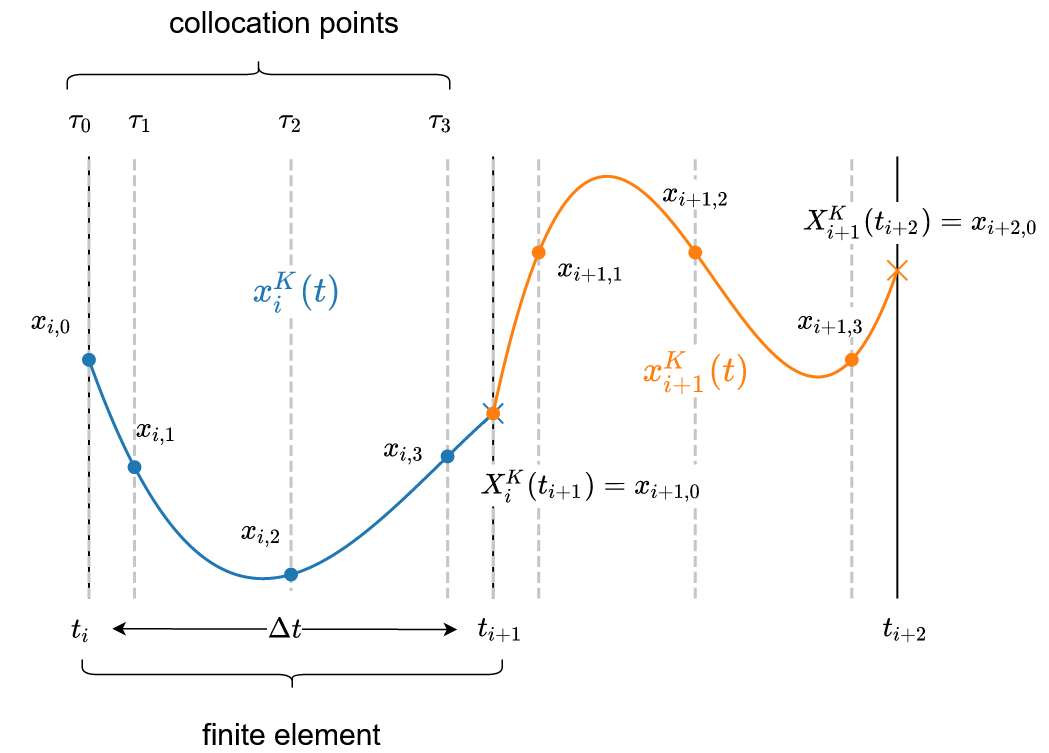
\includegraphics[width=0.95\textwidth]{fig/Collocationdompc}}
    \caption[Beispielhafte orthogonale Kollokation auf finiten Elementen]{Beispielhafte orthogonale Kollokation auf finiten Elementen \cite{Dompc1}}
    \label{fig_Collocationdompc}
\end{figure}

Die erforderliche Steigung der Polynome an den Kollokationspunkten ist durch die Zustandstrajektorien als Optimierungsvariable vorgegeben.
In Abbildung \ref{fig_Collocationdompc} ist zu erkennen, dass auch die Kontinuität der einzelnen Polynome elementübergreifend erfüllt wird, wenn
\begin{equation} \label{eq_KontiDompc}
    \boldsymbol{X}^{K}_{i}(t_{i+1})=\boldsymbol{x}_{i+1,0}
\end{equation}
% \centerline{\small{\textsf{\textbf{Formel \ref{eq_Label}:}} Beschriftung}}
\myequations{\quad Kontinuitätsbedingung der Kollokation im Beispiel der Abbildung \ref{fig_Collocationdompc}}

\vspace*{-\baselineskip}gilt.
Diese Kontinuität gilt jedoch nur für die Zustände und nicht deren zeitliche Ableitungen \cite[S.2]{Cizniar}.

Die Verteilung der Kollokationspunkte innerhalb der finiten Elemente geschieht in der Regel nach vier Methoden \cite[S.48]{Huntington}:
\begin{itemize}
    \item Äquidistant,
    \item Legendre-Gauss,
    \item Legendre-Gauss-Radau,
    \item Legendre-Gauss-Lobatto
\end{itemize}
Äquidistante Verteilungen werden in der Praxis nicht genutzt, je nach Systemdynamik muss zwischen den weiteren Methoden gewählt werden \cite{Huntington}.
Die nachfolgende Abbildung \ref{fig_Kollokationspunkte} zeigt die unterschiedlichen Verteilungen für $K=10$ Kollokationspunkte.

\begin{figure}[h!]
    \centering
    \setlength{\fboxsep}{1pt}
    \setlength{\fboxrule}{1pt}
    \fbox{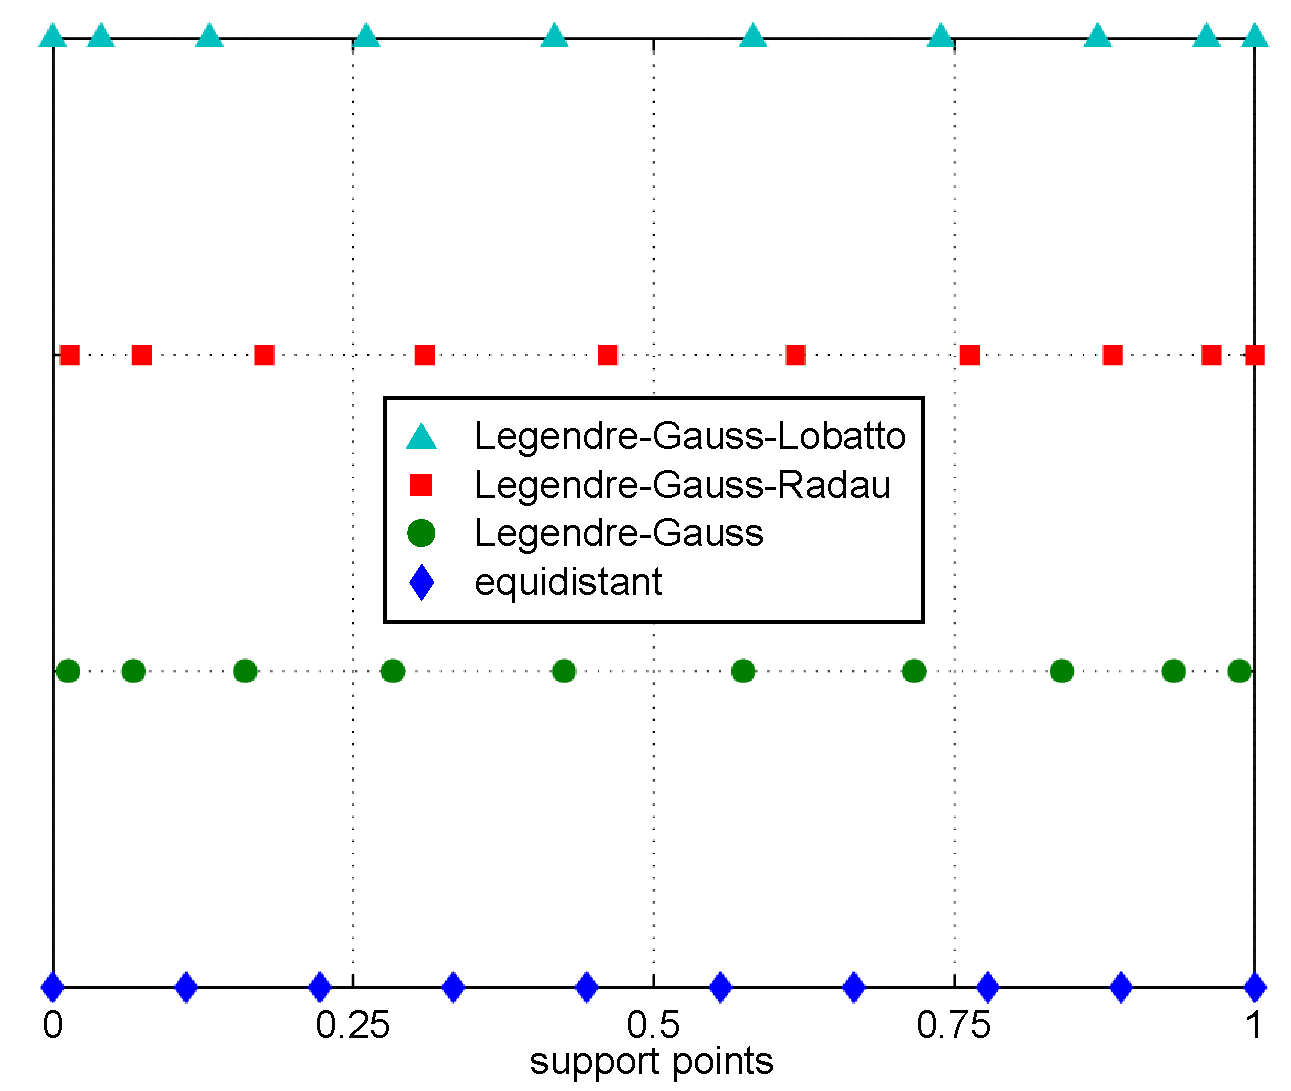
\includegraphics[width=0.9\textwidth]{fig/KollokPoints.pdf}}
    \caption[$K=10$ Kollokationspunkte in Verteilungen nach Legendre-Gauss, Legendre-Gauss-Radau, Legendre-Gauss-Lobatto oder äquidistant im Intervall {$\left[0,1\right]$}]{$K=10$ Kollokationspunkte in Verteilungen nach Legendre-Gauss, Legendre-Gauss-Radau, Legendre-Gauss-Lobatto oder äquidistant im Intervall $\left[0,1\right]$ (gemäß \cite[S.48]{Huntington})}
    \label{fig_Kollokationspunkte}
\end{figure}

Die Approximationspolynome berechnen sich aus
\begin{equation} \label{eq_Approxpolynom2}
\boldsymbol{x}_i^{K}(t)=\sum_{j=0}^K L_j(\tau) \boldsymbol{x}_{i, j},
\end{equation}
% \centerline{\small{\textsf{\textbf{Formel \ref{eq_Label}:}} Beschriftung}}
\myequations{\quad Berechnung der Approximationspolynome}

\vspace*{-\baselineskip}wobei $L_j(\tau)$ das Lagrange-Polynom darstellt, welches nach Gleichung \ref{eq_LagragePloynom} beschrieben wird:
\begin{equation} \label{eq_LagragePloynom}
    \begin{gathered}
        L_j(\tau)=\prod_{\substack{k=0 \\ k \neq j}}^K \frac{\left(\tau-\tau_k\right)}{\left(\tau_j-\tau_k\right)}, \quad \tau=\frac{t-t_i}{\Delta t_i}, \quad \Delta t_i=t_{i+1}-t_i\\
        \forall~i\in \left\{1, \ldots, \mathrm{NE}\right\} \text{ and } j\in \left\{0, \ldots, K\right\}
    \end{gathered}
\end{equation}
% \centerline{\small{\textsf{\textbf{Formel \ref{eq_Label}:}} Beschriftung}}
\myequations{\quad Lagrange-Polynom}

Die zeitliche Ableitung des Polynoms wird wie folgt bestimmt
\begin{equation} \label{eq_AbleitungPolynomKollok}
    \begin{gathered}
        \left.\frac{d \boldsymbol{x}_i^K}{d t}\right|_{t_{i, k}}=\sum_{j=0}^K \frac{\boldsymbol{x}_{i, j}}{\Delta t_i} \underbrace{\left.\frac{d L_j}{d \tau}\right|_{\tau_k}}_{a_{j,k}},\\
        \forall~i\in \left\{1, \ldots, \mathrm{NE}\right\}\text{ and }k\in \left\{0, \ldots, \mathrm{K}\right\}
    \end{gathered}
\end{equation}
% \centerline{\small{\textsf{\textbf{Formel \ref{eq_Label}:}} Beschriftung}}
\myequations{\quad Zeitliche Ableitung des Approximationspolynoms}

\vspace*{-\baselineskip}wobei der Term $a_{j,k}$ konstant ist und vorberechnet werden kann.
Die Erfüllung der Systemdynamiken durch das Polynom an den Kollokationspunkten kann anhand von Gleichheitsbedingungen formuliert werden.
Dabei steht $\boldsymbol{\dot{x}}$ für die durch Differentialgleichungen beschriebene Systemdynamik \cite[S.70]{DissGall}.
\begin{equation} \label{eq_GleichheitsbedAbleitungKollok}
    \begin{gathered}
        \dot{\boldsymbol{x}_i}(\tau) = \sum_{j=0}^K \frac{\boldsymbol{x}_{i, j}}{\Delta t_i} a_{j,k}\\
\forall~i\in \left\{1, \ldots, \mathrm{NE}\right\}\text{ and }k\in \left\{0, \ldots, \mathrm{K}\right\}
    \end{gathered}
\end{equation}
% \centerline{\small{\textsf{\textbf{Formel \ref{eq_Label}:}} Beschriftung}}
\myequations{\quad Gleichheitsbedingungen der Systemdynamik in der Kollokation}

An den Stützstellen der Elemente werden die Gleichheitsbedingungen für die Übergänge der Elemente definiert.
Der Startwert eines Polynoms ist festgelegt durch das Polynom des vorigen Elementes zum Zeitpunkt $\tau=1$, bei dem der Stetigkeitskoeffizient $d_j$ vorberechnet werden kann.
\begin{equation} \label{eq_GleichheitsbedZustandKollok}
    \begin{gathered}
        \boldsymbol{x}_i^K\left(t_{i+1}\right)=\sum_{j=0}^K \underbrace{L_j(\tau=1)}_{d_j} \boldsymbol{x}_{i, j}\\
        \forall~i\in \left\{1, \ldots, \mathrm{NE}\right\}
    \end{gathered}
\end{equation}
% \centerline{\small{\textsf{\textbf{Formel \ref{eq_Label}:}} Beschriftung}}
\myequations{\quad Gleichheitsbedingungen der Übergänge der finiten Elemente}

Die Gleichungen \ref{eq_GleichheitsbedAbleitungKollok} und \ref{eq_GleichheitsbedZustandKollok} werden in das Optimierungsproblem der modellprädiktiven Regelung als Gleichheitsbedingungen eingebunden.


\subsection{Kostenfunktion} \label{subsec_Kostenfunktion}
Liegt dem Regler ein mathematisch hinreichend beschriebenes Modell vor, kann eine sogenannte Kostenfunktion aufgestellt werden, welche die Abweichung zwischen dem vorliegenden und dem gewünschten Systemzustand beschreibt.
Während des Optimierungsprozesses wird die in Abbildung \ref{fig_RegelkreisMPC} dargestellte Optimierungseinheit diese Funktion minimieren und somit den Fehler~$\boldsymbol{e}$ reduzieren.
In der Kostenfunktion sollte der Vergleich der zu regelnden Ausgangsvariablen mit der Referenztrajektorie über den Regelungshorizont abgebildet sein.
Dies geschieht zumeist in quadratischer Form, aufgrund der Differenzierbarkeit und der globalen Konvergenz dieser Gleichungen \cite[S.24]{Diehl}\cite[S.3]{Schwenzer}.
Weiterhin ist es in der Regel zielführend, die errechnete Veränderung der Eingangsvariablen $\Delta \boldsymbol{u}$ zwischen zwei Zeitschritten in die Kostenfunktion mit aufzunehmen, um einem unruhigen Regelverhalten vorzubeugen \cite[S.24]{Diehl}.
Ein mathematisches Beispiel einer solchen Kostenfunktion $\boldsymbol{J}$ ist in Formel \ref{eq_Kostenfunktion} zu sehen; dabei stehen $\boldsymbol{W_w}$ und $\boldsymbol{W_u}$ für Gewichtungsmatrizen und $\boldsymbol{y}(k+i\rvert k)$ für die zum Zeitpunkt $k$ bezüglich des Zeitpunktes $k+i$ vorhergesagte Ausgangsvariable. \cite[S.3]{Schwenzer}

\begin{equation} \label{eq_Kostenfunktion}
\boldsymbol{J}=\sum_{i=N_1}^{N_2}\|\boldsymbol{r}(k+i \mid k)-\boldsymbol{y}(k+i \mid k)\|_{\boldsymbol{W_w}}+\sum_{j=1}^{N_u-1}\|\Delta \boldsymbol{u}(k+j \mid k)\|_{\boldsymbol{W_u}}
\end{equation}
% \centerline{\small{\textsf{\textbf{Formel \ref{eq_Kostenfunktion}:}} Beispielhafte Kostenfunktion für den MPC}}
\myequations{\quad Beispielhafte Kostenfunktion für den MPC}


\subsection{Constraints} \label{subsec_Constraints}
Wie in Abschnitt \ref{subsec_GrundlagenMPC} beschrieben, sind auch die Constraints, also Beschränkungen auf Ein- und Ausgangsgrößen des Systems, ein wesentliches Merkmal modellprädiktiver Regelung.
Während der Optimierung der Kostenfunktion wird bei Einbindung von Constraints sichergestellt, dass beispielsweise mechanische oder physikalische Limitierungen des Systems nicht überschritten werden.
Dabei ist zwischen den sogenannten \textit{hard constraints} und \textit{soft constraints} zu unterscheiden.
Nicht zu überschreitende, harte Limitierungen treten zumeist bei den Eingangsgrößen auf; beispielhaft kann das maximale Drehmoment eines Motors genannt werden.
Im Gegensatz dazu sind harte Beschränkungen auf Ausgangsgrößen oft nur gewünscht als wirklich erforderlich und können das Optimierungsproblem unlösbar machen.
Dies geschieht, wenn die limitierten Eingangsgrößen das System nicht auf eine Weise beeinflussen können, dass die Ausgangsgrößen ihren vorgegebenen Rahmen beibehalten.
Ein zusätzlicher Freiheitsgrad wird durch die Einführung von soft constraints und sogenannten \textit{Slack Variablen} $\boldsymbol{\xi}$ geschaffen. \cite[S.4]{Schwenzer}

Mathematisch lässt sich die in Gleichung \ref{eq_Kostenfunktion} dann um die constraints und die Gleichheitsbedingungen aus Gleichung \ref{eq_GleichheitsbedAbleitungKollok} und \ref{eq_GleichheitsbedZustandKollok} auf das gesamte Optimierungsproblem erweitern.
Dazu wird nach \cite[S.4]{Schwenzer} eine weitere Gewichtungsmatrix $\boldsymbol{W_\xi}$ in der Kostenfunktion eingefügt, um Dauer und Höhe der constraint-Überschreitung zu beeinflussen \cite{Rawlings}.
Die Indizes \textit{lb} und \textit{ub} kennzeichnen die \textbf{l}ower bzw. \textbf{u}pper \textbf{b}ound, also die untere und obere Variablengrenze.
Die für die Diskretisierung eingeführten Indizes werden mit \textit{col} erweitert.

\begin{equation} \label{eq_Optimierungsproblem}
\begin{gathered}
\min_{\boldsymbol{x}, \boldsymbol{u}, \boldsymbol{\xi}, t} \quad \sum_{i=N_1}^{N_2}\|\boldsymbol{r}(k+i \mid k)-\boldsymbol{y}(k+i \mid k)\|_{\boldsymbol{W_w}}+\sum_{j=1}^{N_u-1}\|\Delta \boldsymbol{u}(k+j \mid k)\|_{\boldsymbol{W_u}}+\sum_{i=N_1}^{N_2}\|\boldsymbol{\xi}(k+i \mid k)\|_{\boldsymbol{W_{\xi}}} \qquad\\
\dot{\boldsymbol{x}}_{i_{\mathrm{col}}}(\tau) - \sum_{j_{\mathrm{col}}=0}^K \frac{\boldsymbol{x}_{i_{\mathrm{col}}, j_{\mathrm{col}}}}{\Delta t_{i_{\mathrm{col}}}} a_{j_{\mathrm{col}},k_{\mathrm{col}}} = \mathbf{0}\\
\boldsymbol{x}_{i_{\mathrm{col}}}^K\left(t_{i_{\mathrm{col}}+1}\right) -\sum_{j_{\mathrm{col}}=0}^K d_{j_{\mathrm{col}}} \boldsymbol{x}_{i_{\mathrm{col}}, j_{\mathrm{col}}} = \mathbf{0}\\
\boldsymbol{u}_{l b} \leq(\boldsymbol{u}(k+j \mid k)) \leq \boldsymbol{u}_{u b}, \\
\boldsymbol{y}_{l b}-(\boldsymbol{\xi}(k+i \mid k)) \leq(\boldsymbol{y}(k+j \mid k)) \leq \boldsymbol{y}_{u b}+(\boldsymbol{\xi}(k+i \mid k)), \\
\forall~\tau \in \left[0,1\right] \text{, } i_{\mathrm{col}} \in \left\{1, \ldots, \mathrm{NE}\right\} \text{ and } k_{\mathrm{col}} \in \left\{0, \ldots, \mathrm{K}\right\}\\
\forall~\boldsymbol{\xi} \geq \mathbf{0} \text{, }i \in\left\{N_1, \ldots, N_2-i\right\} \text { and } j \in\left\{0, \ldots, N_u\right\}
\end{gathered}
\end{equation}

\vspace*{-10\baselineskip}
\qquad subject to:
\vspace*{9\baselineskip}
\myequations{\quad Beispielhaftes Optimierungsproblem für den MPC}
% \centerline{\small{\textsf{\textbf{Formel \ref{eq_Optimierungsproblem}:}} Beispielhaftes Optimierungsproblem für den MPC}}

Eine gut konstruierte Kostenfunktion ermöglicht es, das Ziel des Modells oder Systems präzise zu definieren, unerwünschte Effekte oder Fehler zu minimieren und die gewollten Ergebnisse zu erzielen.
Dazu sind die Zielvariablen, die Gewichtungen und die constraints sinnvoll zu wählen.

\section{Modellbildung des offen volumetrischen Receivers} \label{sec_Ausgangszustand}
In \cite[S.90ff]{DissGall} wird die Modellierung der Absorbercups im Receiver am Solarturm Jülich vorgestellt und in \cite{IdingSolarPaces} erweitert.
Die jeweiligen Ergebnisse werden an dieser Stelle verknüpft.
Die Modellierung hat das Ziel eine einfache mathematische Beschreibung des Receivers zu erreichen, um für Optimierungszwecke geeignet zu sein.
Ausgehend vom aufgeprägten Massenstrom, der Temperatur der Rückführluft und Umgebung sowie der solaren Einstrahlung soll das Verhalten des Receivers, insbesondere die Luftaustrittstemperatur und die Oberflächentemperatur, hinreichend genau abbildet werden \cite[S.90]{DissGall}.

\subsection{Grundlagen und Annahmen} \label{subsec_GrundlagenAnnahmen}
Die modellierte Receiver Front besteht aus einzelnen \textit{Absorbercups}.
Es wird davon ausgegangen, dass die einzelnen Cups nicht miteinander interagieren, das heißt thermisch voneinander isoliert sind \cite[S.91]{DissGall}.
Die Cups selbst bestehen aus drei Komponenten, wie in Abbildung \ref{fig_AufbauCup} zu sehen ist.

\begin{figure}[h!]
    \centering
    \setlength{\fboxsep}{1pt}
    \setlength{\fboxrule}{1pt}
\fbox{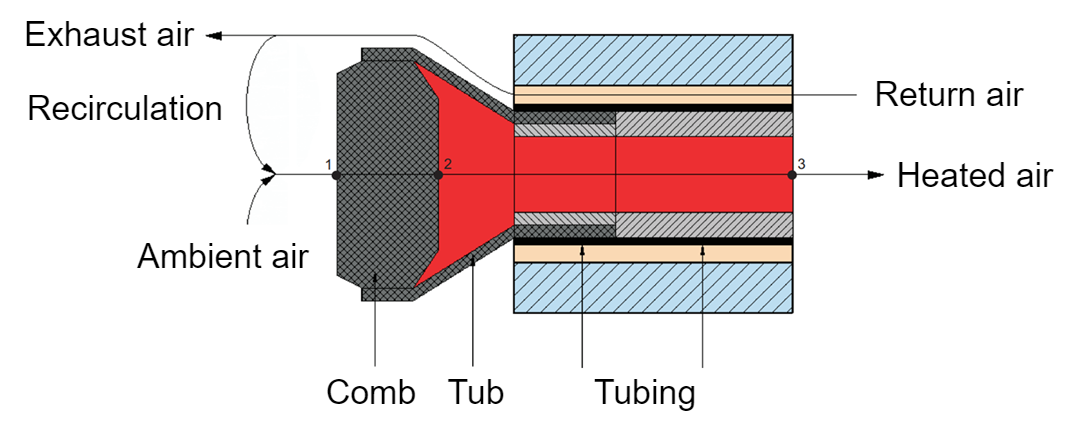
\includegraphics[width=0.9\textwidth]{fig/AbsorberCupE2}}
    \caption[Schematische Darstellung eines Absorbercups]{Schematische Darstellung eines Absorbercups (nach \cite[S.90]{DissGall})}
    \label{fig_AufbauCup}
\end{figure}

Die dargestellten Komponenten sind:
\begin{itemize}
    \item \textbf{Absorberwabe} (\textit{Comb}): Sie besteht aus einer porösen Keramik und dient der Absorption der konzentrierten Solarstrahlung.
          Diese wird in der Keramik in thermische Energie gewandelt und als innere Energie gespeichert.
          Aufgrund der porösen Struktur kann Umgebungsluft als Wärmeübertragungsmedium durch die Wabe strömen, die Energie aufnehmen und diese dem nachgeschalteten Prozess (vgl. Abschnitt \ref{sec_Solartürme}) zur Verfügung stellen.
    \item \textbf{Absorberkelch} (\textit{Tub}): Er besteht aus demselben Material wie die Absorberwabe, ist jedoch massiv.
          Der Kelch ist wie ein quadratischer Pyramidenstumpf mit rundem Auslass geformt und sammelt die warme Luft nach Durchströmen der Wabe.
    \item \textbf{Rohrstück} (\textit{Tubing}): Dieses dient dem Transport der Luft zur weiteren Nutzung. Der vordere Teil des Rohrs besteht neben der Isolierung aus dem Endstück des Kelches. Am Ende des Rohrstücks befindet sich eine Blende, die je nach Position des Cups im Receiver einen unterschiedlichen Durchmesser besitzt.
\end{itemize}

Zur Erhöhung des Wirkungsgrades des Receivers wird die abgekühlte Luft (rund \SIrange{80}{120}{\degreeCelsius}) \cite{IdingSolarPaces} aus dem Prozess zu den Absorbercups zurückgeführt.
Dort wird sie in Luftschlitzen zwischen den einzelnen Cups vor den Receiver geleitet, wo sie sich teilweise mit der Umgebungsluft mischt und erneut für die Wärmeübertragung zur Verfügung steht.
Dieser Prozess ist in Abbildung \ref{fig_AufbauCup} dargestellt.

Die Cups werden in vier Sektoren unterteilt, welchen jeweils ein sogenannter primärer \textit{Header} nachgeschaltet ist.
In diesen Headern wird die aus dem Rohrstück jedes einzelnen Cups austretende, erwärmte Luft gemischt und ein bezüglich der Temperatur homogenisierter Luftmassenstrom entsteht.
Über ein Ventil am Luftaustrittspunkt der Header kann theoretisch der Luftstrom durch die einzelnen Sektoren reguliert werden.
In der Praxis ist dieses Ventil jederzeit geöffnet \cite{IdingSolarPaces}.
An die vier primären Header schließt sich ein sekundärer Header an, welcher den identischen homogenisierenden Effekt mit der Luft aus allen vier Sektoren, also dem gesamten Luftmassenstrom des Receivers, erzielt.
Die schematische Darstellung zeigt Abbildung \ref{fig_HeaderSchema}.

\begin{figure}[h!]
    \centering
    \setlength{\fboxsep}{8pt}
    \setlength{\fboxrule}{1pt}
    \fbox{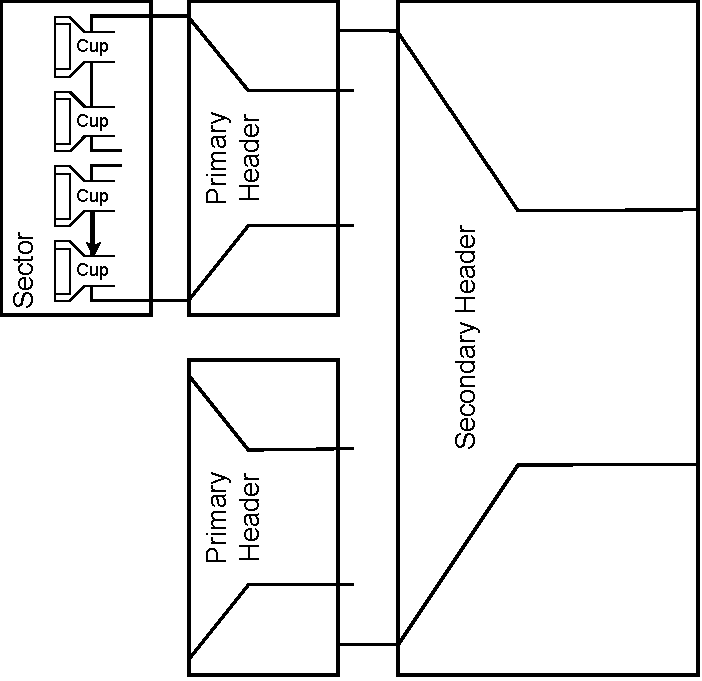
\includegraphics[width=0.55\textwidth]{fig/Header_Darstellung}}
    \caption[Schematische Darstellung der Header]{Schematische Darstellung der Header (nach \cite[S.90]{DissGall})}
    \label{fig_HeaderSchema}
\end{figure}

Um das Modell des Receivers einfach zu halten, werden die folgenden Annahmen getroffen \cite[S.92]{DissGall}:
\begin{itemize}
\item Die einzelnen Absorbercups sind thermisch voneinander isoliert.
\item Das System wird als isobar angenommen, sodass die Enthalpie der Luft ausschließlich von der Temperatur abhängt.
    \item Die Lufttemperaturen innerhalb von Bilanzräumen sind homogen und ändern sich diskret an Bilanzgrenzen.
    \item Die Temperaturen der Rückführluft und der Luft hinter der Absorberwabe sind homogen.
Dadurch wird die Berechnung der Wärmeübertragung vereinfacht, ohne die Genauigkeit der Berechnung zu stark zu beeinflussen, da die lokalen Temperaturänderungen relativ gering sind.
    \item Die Absorberwabe ist die einzige Komponente, die Wärme speichert.
\end{itemize}


\subsection{Modellierung eines Absorbercups} \label{subsec_ModellCup}
Zur Berechnung der Entahlpieströme und Temperaturen kann der Absorbercup vereinfacht in die Aufheizzone, (gemäß o.g. Annahme: die Wabe), und die Transportzone (Kelch und Rohrstück), aufgeteilt werden.
Die real auftretenden Temperaturunterschiede zwischen Kelch und Rohrstrück sind vernachlässigbar gering, sodass eine Einzelbetrachtung dieser beiden Komponenten nicht erforderlich ist \cite[S.93]{DissGall}.
Abbildung \ref{fig_AbsorberBerechnung} zeigt die beiden Zonen und alle Größen zur nachfolgenden Berechnung.

\begin{figure}[h!]
    \centering
    \setlength{\fboxsep}{1pt}
    \setlength{\fboxrule}{1pt}
\fbox{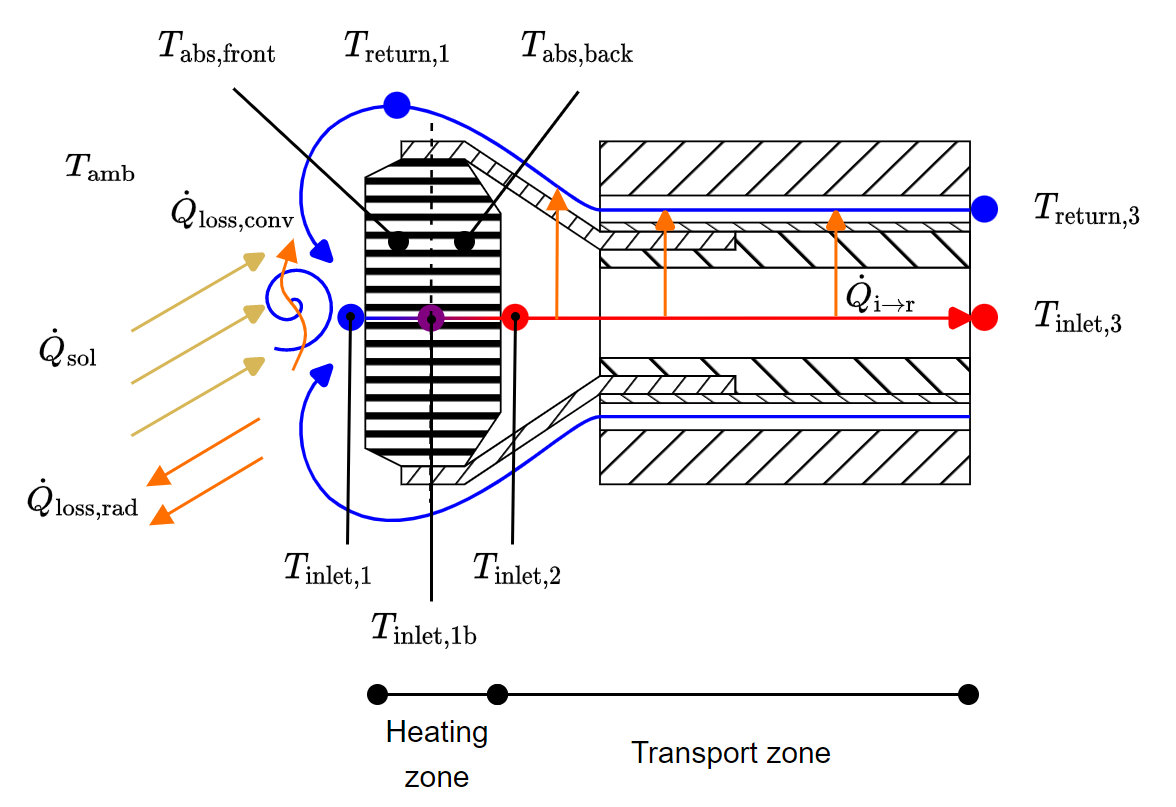
\includegraphics[width=1\textwidth]{fig/AbsorberCupGleichungen_new}}
    \caption[Berechnungsgrößen des Absorbercups]{Berechnungsgrößen des Absorbercups (nach \cite{IdingSolarPaces})}
    \label{fig_AbsorberBerechnung}
\end{figure}

\subsubsection*{Aufheizzone} \label{subsubsec_EnergiebilanzAufheizzone}
Gemäß Abbildung \ref{fig_AbsorberBerechnung} ergibt sich die Energiebilanz an der Vorderseite der Absorberwabe zu
\begin{equation} \label{eq_EnergiebilanzWabe}
\UDotAbsorberFront =\QDotSolFront - \QDotLossAbsorberCupConvective -  \QDotLossAbsorberCupRadiative -\QDotAbsorberCombFront - \QDotConduction,
\end{equation}
% \centerline{\small{\textsf{\textbf{Formel \ref{subsubsec_EnergiebilanzAufheizzone}:}} Energiebilanz der Absorberwabe}}
\myequations{\quad Energiebilanz der Vorderseite der Absorberwabe}

\vspace*{-\baselineskip}wobei $\UDotAbsorberFront$ die Änderung der inneren Energie der Wabenfront und $\QDotSolFront$ die von ihr aufgenommene solare Einstrahlung beschreibt.
Die Terme $\QDotLossAbsorberCupConvective$ und $\QDotLossAbsorberCupRadiative$ beschreiben die thermischen Verluste in Folge von Wind und Wärmestrahlung.
Der gewünschte Wärmeübergang von der Wabe in die durchströmende Luft wird mit $\QDotAbsorberCombFront$ ausgedrückt.
$\QDotConduction$ steht für die Wärmeleitung des vorderen Teils der Wabe in den hinteren Teil.\\
Die Änderung der inneren Energie kann weiterhin ausgedrückt werden als
\begin{equation} \label{eq_InnereEnergie}
\UDotAbsorberFront = m_{\mathrm{abs,front}} \cdot c_{\mathrm{abs}} \cdot \frac{d \TAbsorberFront}{d t},
\end{equation}
% \centerline{\small{\textsf{\textbf{Formel \ref{eq_InnereEnergie}:}} Änderung der inneren Energie der Absorberfornt}}
\myequations{\quad Änderung der inneren Energie der Absorberfront}

\vspace*{-\baselineskip}mit der Masse des vorderen Absorberwabenteils $m_{\mathrm{abs,front}}$ und der Wärmekapazität $c_{\mathrm{abs}}$, sowie der Änderung der Fronttemperatur über die Zeit.

Aufgrund der Struktur der Absorberwaben wird nicht die gesamte Einstrahlungsleistung an der Vorderseite der Wabe aufgenommen.
Dies wird mit dem Faktor $\xi_{\mathrm{rad}}$ berücksichtigt, welcher diese Leistung in zwei Teile trennt.
\begin{equation} \label{eq_SolareLeistung}
    \begin{aligned}
        \PowerSolarFront & = \xi_{\mathrm{rad}} \PowerSolar     \\
        \PowerSolarBack  & = (1-\xi_{\mathrm{rad}}) \PowerSolar
    \end{aligned}
\end{equation}
% \centerline{\small{\textsf{\textbf{Formel \ref{eq_SolareLeistung}:}} Einteilung der aufgenommenen solaren Leistung mittels $\xi_{\mathrm{rad}}$}}
\myequations{\quad Einteilung der aufgenommenen solaren Leistung mittels $\xi_{\mathrm{rad}}$}

Mit der an der Wabenvorderseite aufgenommenen Leistung und dem Absorptionskoeffizienten $\alpha_{\mathrm{sol}}$ sowie der Absorberoberfläche $\SurfaceFront$ und der Flussdichte $\FluxSolar$ ergibt sich
\begin{equation} \label{eq_SolareEinstrahlung}
\QDotSolFront = \alpha_{\mathrm{sol}} \PowerSolarFront = \alpha_{\mathrm{sol}} \xi_{\mathrm{rad}} \SurfaceFront \FluxSolar.
\end{equation}
% \centerline{\small{\textsf{\textbf{Formel \ref{eq_SolareEinstrahlung}:}} Absorbierte solare Einstrahlung an der Wabenfront}}
\myequations{\quad Absorbierte solare Einstrahlung an der Wabenfront}

Zu einem Zeitpunkt, wenn kein Wind den Receiver beeinträchtigt, sind die thermischen Verluste durch Konvektion $\QDotLossAbsorberCupConvective$ nicht vorhanden.
Da außerdem die explizite Betrachtung dieser Verluste sehr komplex ist und ein eigenes Forschungsfeld darstellt, werden diese Verluste nicht weiter betrachtet \cite{IdingSolarPaces}. Damit gilt:
\begin{equation} \label{eq_KonvektiveVerluste}
\QDotLossAbsorberCupConvective = 0.
\end{equation}
% \centerline{\small{\textsf{\textbf{Formel \ref{eq_KonvektiveVerluste}:}} Bestimmung der Verluste durch Konvektion}}
\myequations{\quad Bestimmung der Verluste durch Konvektion}

Die Verluste durch Wärmestrahlung können mit dem Stefan-Boltzmann-Gesetz beschrieben werden.
Dabei ist $\epsilon$ der Emissionskoeffizient, welcher zur Vereinfachung gleich dem Absorptionskoeffizienten $\alpha_{\mathrm{sol}}$ gesetzt wird, $\sigma$ die Boltzmann-Konstante und $\TAmbient$ die Umgebungstemperatur. Somit ergibt sich:
\begin{equation} \label{eq_StrahlungVerluste}
    \QDotLossAbsorberCupRadiative = \epsilon \sigma \SurfaceFront (\TAbsorberFront^4-\TAmbient^4)
\end{equation}
% \centerline{\small{\textsf{\textbf{Formel \ref{eq_Label}:}} Beschriftung}}
\myequations{\quad Bestimmung der Verluste durch Wärmestrahlung}

Die Konvektion an der Vorderseite der Absorberwabe auf die durchströmende Luft kann durch die Enthalpieströme beschrieben werden.
Weiterhin ist auch die Berechnung mit dem Wärmeübergangskoeffizienten $\HeatTransferCoefficientAbsorberFront$ und der Kontaktfläche zwischen Luft und Absorberwabe $\HeatTransferSurfaceFront$ möglich:
\begin{equation} \label{eq_gewünschteKonvektion}
    \begin{aligned}
        \QDotAbsorberCombFront & = \EnthalpyFlowTInlet{\mathrm{1b}} - \EnthalpyFlowTInlet{1}                                              \\
                               & = \MDotAbsorberCup \cdot ( \SpecificEnthalpyTInlet{\mathrm{1b}} - \SpecificEnthalpyTInlet{1})            \\
                               & = \HeatTransferCoefficientAbsorberFront \HeatTransferSurfaceFront (\TAbsorberFront-T_{\mathrm{m,front}})
    \end{aligned}
\end{equation}
% \centerline{\small{\textsf{\textbf{Formel \ref{eq_Label}:}} Beschriftung}}
\myequations{\quad Konvektion zwischen Wabenfront und Luftmassenstrom}

Für diese Berechnung wird die Durchschnittstemperatur $T_{\mathrm{m,front}}$ zwischen dem Lufteintritt $\TInlet{1}$ und der Mitte der Wabe $\TInlet{1b}$ mit dem einstellbaren Gewichtungsfaktor $\TemperatureWeightingFactor$ genutzt, welche sich gemäß Gleichung \ref{eq_MeanTempAbsFront} ergibt.
\begin{equation} \label{eq_MeanTempAbsFront}
    T_{\mathrm{m,front}} = (1-\TemperatureWeightingFactorFront) \TInlet{1} + \TemperatureWeightingFactorFront \TInlet{\mathrm{1b}}
\end{equation}
% \centerline{\small{\textsf{\textbf{Formel \ref{eq_Label}:}} Beschriftung}}
\myequations{\quad Berechnung der durchschnittlichen Temperatur in der Wabenfront}

Die Wärmeleitung von der Absorbervorderseite zur -rückseite ergibt sich unter Berücksichtigung der Wärmeleitfähigkeit $\lambda_{\mathrm{comb}}$, $\SurfaceFrontSolid$ als Oberfläche der Absorberfront abzüglich der Fläche für die Luftschlitze und $l_{\mathrm{comb}}$ als Tiefe des Absorbers:
\begin{equation} \label{eq_WärmeleitungVorneHinten}
\QDotConduction = \lambda_{\mathrm{comb}} \cdot \frac{\SurfaceFrontSolid \cdot (\TAbsorberFront-\TAbsorberBack)}{\frac{l_{\mathrm{comb}}}{2}}
\end{equation}
% \centerline{\small{\textsf{\textbf{Formel \ref{eq_Label}:}} Beschriftung}}
\myequations{\quad Wärmeleitung der Absorbervorderseite zur -rückseite}

\vspace*{-\baselineskip}Durch die Halbierung der Absorbertiefe wird gewährleistet, dass die Betrachtung die Wärmeleitung zwischen der Mitte der Absorberfront und der Mitte der Rückseite betrachtet wird.

Für die hintere Seite der Absorberwabe kann eine der Gleichung \ref{eq_EnergiebilanzWabe} ähnliche Energiebilanz aufgestellt werden.
Allerdings wird an dieser Stelle kein Verlust durch Wärmestrahlung beachtet, da die Oberfläche der Wabenrückseite größtenteils dem Kelch und nicht der Umgebung zugewandt ist und daher der Anteil an Strahlungsverlusten an die Umgebung vernachlässigbar ist:
\begin{equation} \label{eq_EnergiebilanzWabeHinten}
    \UDotAbsorberBack =\QDotSolBack -\QDotAbsorberCombBack + \QDotConduction
\end{equation}
% \centerline{\small{\textsf{\textbf{Formel \ref{eq_Label}:}} Beschriftung}}
\myequations{\quad Energiebilanz der Rückseite der Absorberwabe}

$\QDotAbsorberCombBack$ kann dabei wie folgt beschrieben werden:
\begin{equation} \label{eq_KonvektionWabeHinten}
    \begin{aligned}
        \QDotAbsorberCombBack & = \EnthalpyFlowTInlet{2} - \EnthalpyFlowTInlet{\mathrm{1b}}                                          \\
                              & = \MDotAbsorberCup \cdot ( \SpecificEnthalpyTInlet{2} - \SpecificEnthalpyTInlet{\mathrm{1b}})        \\
                              & = \HeatTransferCoefficientAbsorberBack \HeatTransferSurfaceBack (\TAbsorberBack-T_{\mathrm{m,back}})
    \end{aligned}
\end{equation}
\myequations{\quad Konvektion zwischen Wabenfront und Luftmassenstrom}

Die durchschnittliche Temperatur an der Rückseite der Absorberwabe errechnet sich nach Gleichung \ref{eq_MeanTempAbsBack}.
\begin{equation} \label{eq_MeanTempAbsBack}
    T_{\mathrm{m,back}}  = (1-\TemperatureWeightingFactorBack) \TInlet{\mathrm{1b}} + \TemperatureWeightingFactorBack \TInlet{2}
\end{equation}
% \centerline{\small{\textsf{\textbf{Formel \ref{eq_Label}:}} Beschriftung}}
\myequations{\quad Berechnung der durchschnittlichen Temperatur in der Wabenrückseite}

Durch Erweiterung von Gleichung \ref{eq_EnergiebilanzWabe} um die Gleichungen \ref{eq_InnereEnergie} bis \ref{eq_WärmeleitungVorneHinten} erhält man folgende Differentialgleichung für die vordere Seite der Absorberwabe:
\setlength{\eqlinespacing}{25pt}
\begin{dmath} \label{eq_GesamtgleichungEnergiebilanzWabeVorne}
    m_{\mathrm{abs,front}}  c_{\mathrm{abs}} \frac{d \TAbsorberFront}{d t} = \epsilon \xi_{\mathrm{rad}} \SurfaceFront \FluxSolar -  \epsilon \sigma \SurfaceFront (\TAbsorberFront^4-\TAmbient^4) - \HeatTransferCoefficientAbsorberFront \HeatTransferSurfaceFront (\TAbsorberFront-T_{\mathrm{m,front}}) - \lambda_{\mathrm{comb}} \cdot \frac{\SurfaceFrontSolid \cdot (\TAbsorberFront-\TAbsorberBack)}{l_{\mathrm{comb}/2}}
\end{dmath}
% \centerline{\small{\textsf{\textbf{Formel \ref{eq_Label}:}} Beschriftung}}
\myequations{\quad Gesamtgleichung der Energiebilanz an der Wabenvorderseite}

Für den hinteren Teil der Wabe ergibt sich aus den Gleichungen \ref{eq_EnergiebilanzWabeHinten} bis \ref{eq_MeanTempAbsBack} eine weitere Differentialgleichung:
\setlength{\eqlinespacing}{25pt}
\begin{dmath} \label{eq_GesamtgleichungEnergiebilanzWabeHinten}
    m_{\mathrm{abs,back}}  c_{\mathrm{abs}} \frac{d \TAbsorberBack}{d t} = \epsilon (1-\xi_{\mathrm{rad}}) \SurfaceFront \FluxSolar \qquad \qquad \qquad \qquad -  \HeatTransferCoefficientAbsorberBack \HeatTransferSurfaceBack (\TAbsorberBack-T_{\mathrm{m,back}}) + \lambda_{\mathrm{comb}} \cdot \frac{\SurfaceFrontSolid \cdot (\TAbsorberFront-\TAbsorberBack)}{l_{\mathrm{comb}/2}}
\end{dmath}
% \centerline{\small{\textsf{\textbf{Formel \ref{eq_Label}:}} Beschriftung}}
\myequations{\quad Gesamtgleichung der Energiebilanz an der Wabenrückseite}


Die Temperaturen $\TAbsorberFront$ und $\TAbsorberBack$ stellen dabei die Systemzustände dar; die Flussdichte $\FluxSolar$ eine Eingangsgröße.
Weiterhin unbekannt sind die Temperaturen $\TInlet{1}$, $\TInlet{1b}$ und $\TInlet{2}$.

$\TInlet{1}$ ergibt sich aus der Energiebilanz vor der Absorberwabe (siehe Abbildung \ref{fig_AbsorberBerechnung}), bei der $arr$ für die Rückführrate der Luft (\textit{air return ratio}) steht.
Dies ist der Anteil, der in den Absorber strömenden Luft, der zuvor aus dem Prozess zurückgeführt wurde.
\begin{equation} \label{eq_EnergiebilanzVorWabe}
    \EnthalpyFlowTInlet{1} = arr \cdot \EnthalpyFlowTReturn{1} + (1-arr) \cdot \EnthalpyFlowTAmbient
\end{equation}
% \centerline{\small{\textsf{\textbf{Formel \ref{eq_Label}:}} Beschriftung}}
\myequations{\quad Energiebilanz vor der Absorberwabe}

Diese Gleichung kann zu
\begin{equation} \label{eq_EnergiebilanzVorWabe2}
    \SpecificEnthalpyTInlet{1} = arr \cdot \SpecificEnthalpyTReturn{1} + (1-arr) \cdot \SpecificEnthalpyTAmbient
\end{equation}
% \centerline{\small{\textsf{\textbf{Formel \ref{eq_Label}:}} Beschriftung}}
\myequations{\quad Transformierte Energiebilanz vor der Absorberwabe}

\vspace*{-\baselineskip}umgeschrieben werden.

Um auf Basis der spezifischen Enthalpie die Temperatur zu bestimmen wird ein Approximationspolynom dritten Grades der Form $T=f(h)$ verwendet.
Dies ist zulässig, da das Approximationspolynom im relevanten Bereich streng monoton steigend ist und so eine geschlossene Lösung erlaubt.
Dies verringert den Rechenaufwand gegenüber anderen Berechnungen, die die temperaturabhängige Wärmekapazität für diese Umrechnung nutzen \cite[S.96]{DissGall}.
Aus Gleichung \ref{eq_EnergiebilanzVorWabe2} ergibt sich mit $\SpecificEnthalpyTReturn{1}$ eine neue Unbekannte, die aus der Energiebilanz der Transportzone errechnet wird.


\subsubsection*{Transportzone} \label{subsubsec_EnergiebilanzTransportzone}
Nach Abbildung \ref{fig_AbsorberBerechnung} ergibt sich die Energiebilanz der Transportzone zu
\begin{equation} \label{eq_EnergiebilanzTransportzone}
\EnthalpyFlowTReturn{1} = \EnthalpyFlowTReturn{3} +\QDotLossAbsorberCupInternal,
\end{equation}
% \centerline{\small{\textsf{\textbf{Formel \ref{eq_Label}:}} Beschriftung}}
\myequations{\quad Energiebilanz der Transportzone}

\vspace*{-\baselineskip}was gleichbedeutend mit
\begin{equation} \label{eq_EnergiebilanzTransportzone2}
    \MDotAbsorberCup\SpecificEnthalpyTReturn{1} = \MDotAbsorberCup\SpecificEnthalpyTReturn{3}+\QDotLossAbsorberCupInternal
\end{equation}
% \centerline{\small{\textsf{\textbf{Formel \ref{eq_Label}:}} Beschriftung}}
\myequations{\quad Energiebilanz der Transportzone (Ausdruck mit spezifischer Enthalpie)}

\vspace*{-\baselineskip}ist, wobei $\QDotLossAbsorberCupInternal$ den Verlustwärmestrom darstellt, der sich nach Abbildung \ref{fig_AbsorberBerechnung} aus drei in orange gekennzeichneten Teilen zusammensetzt und von der Rückführluft aufgenommen wird.
Mathematisch lässt sich dies nach Gleichung \ref{eq_VerlustwärmeTransportzone} beschreiben.
\begin{equation} \label{eq_VerlustwärmeTransportzone}
    \QDotLossAbsorberCupInternal = \QDotLoss{tub} + \QDotLoss{tube,1} + \QDotLoss{tube,2}
\end{equation}
% \centerline{\small{\textsf{\textbf{Formel \ref{eq_Label}:}} Beschriftung}}
\myequations{\quad Aufteilung des Verlustwärmestroms der Transportzone}

Der Wärmeverlust durch die Rohrstücke kann mittels herkömmlicher Formeln der Wärmeübertragung in mehrschichtigen Rohre beschrieben werden.
Durch die Umrechnung des Kelches in ein äquivalentes Rohr können die identischen Formeln auch hier angewandt werden.
Daher gilt
\begin{equation} \label{eq_VerlustwärmeTransportzone2}
\QDotLossAbsorberCupInternal= \alpha_{\mathrm{i\to r}} \cdot A_{\mathrm{i\to r}} \cdot (\TInlet{2} - \TReturn{3}),
\end{equation}
% \centerline{\small{\textsf{\textbf{Formel \ref{eq_Label}:}} Beschriftung}}
\myequations{\quad Berechnung des Verlustwärmestroms der Transportzone}

\vspace*{-\baselineskip}wobei $\alpha_{\mathrm{i\to r}}$ der Wärmeübergangskoeffizient und $A_{\mathrm{i\to r}}$ die entsprechende Kontaktfläche ist.
Die Geometrie des Absorbers zeigt die Abbildung \ref{fig_GeometrieAbsorber}.

\begin{figure}[h!]
    \centering
    \setlength{\fboxsep}{1pt}
    \setlength{\fboxrule}{1pt}
    \fbox{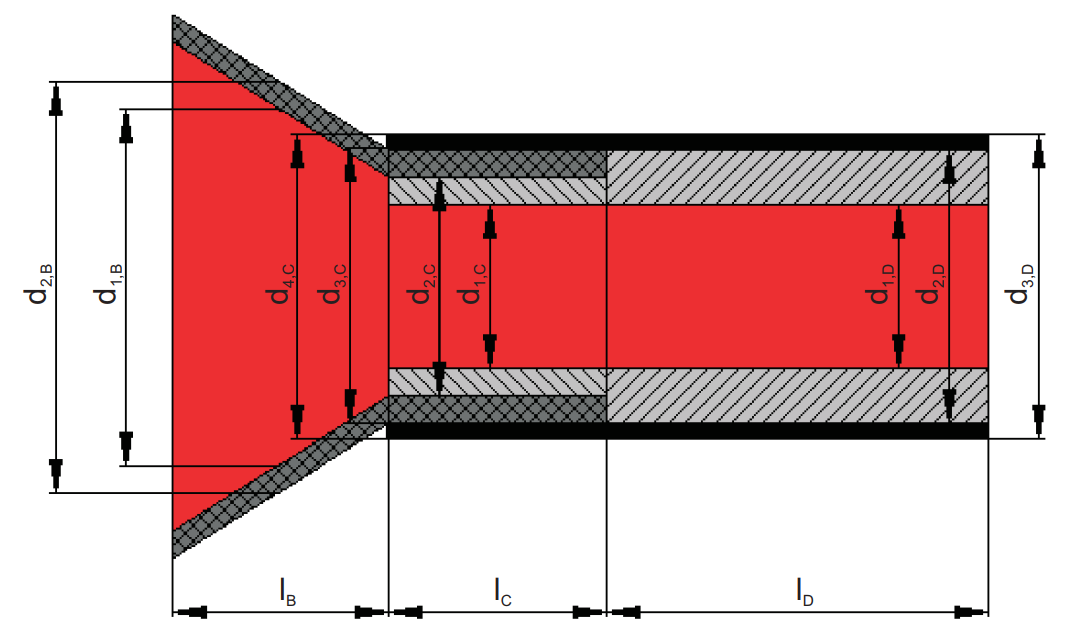
\includegraphics[width=0.8\textwidth]{fig/GeometrieAbsorber}}
    \caption[Geometrie des Absorbers]{Geometrie des Absorbers \cite[S.97]{DissGall}}
    \label{fig_GeometrieAbsorber}
\end{figure}

Aus der Geometrie und den Wärmeleitfähigkeiten $\lambda$ der Keramik, der Dämmung und des Rohres sowie den lokalen Wärmeübergangskoeffizienten ergibt sich
\begin{equation}
\begin{aligned} \label{eq_WärmeübergangskoeffizientVerluste}
\alpha_{\mathrm{i\to r}} & =\frac{\pi \cdot l_{\mathrm{B}}}{\frac{1}{\alpha_{\mathrm{inlet, 2}} \cdot d_{1, \mathrm{B}}}+\frac{1}{2} \cdot B+\frac{1}{\alpha_{\mathrm{return, 3}} \cdot d_{2, \mathrm{~B}}}} \\
& +\frac{\pi \cdot l_{\mathrm{C}}}{\frac{1}{\alpha_{\mathrm{inlet, 2}} \cdot d_{1, \mathrm{C}}}
        +\frac{1}{2} \cdot C+\frac{1}{\alpha_{\mathrm{return, 3}} \cdot d_{4, \mathrm{C}}}}
\\
& +\frac{\pi \cdot l_{\mathrm{D}}}{\frac{1}{\alpha_{\mathrm{inlet, 2}} \cdot d_{1, \mathrm{D}}}+\frac{1}{2} \cdot D+\frac{1}{\alpha_{\mathrm{return, 3}} \cdot d_{3, \mathrm{D}}}},
\end{aligned}
\end{equation}
% \centerline{\small{\textsf{\textbf{Formel \ref{eq_Label}:}} Beschriftung}}
\myequations{\quad Bestimmung Wärmeübergangskoeffizienten für den Verlustwärmestrom}

\vspace*{-\baselineskip}mit
\begin{equation}
\begin{aligned} \label{eq_BestimmungHilfsgrößen}
& B=\frac{1}{\lambda_{\text {cer}}} \cdot \ln \frac{d_{2, \mathrm{B}}}{d_{1, \mathrm{B}}}                                                                                                                                                                              \\
& C=\frac{1}{\lambda_{\text {ins}}} \cdot \ln \frac{d_{2, \mathrm{C}}}{d_{1, \mathrm{C}}}+\frac{1}{\lambda_{\text {cer}}} \cdot \ln \frac{d_{3, \mathrm{C}}}{d_{2, \mathrm{C}}}+\frac{1}{\lambda_{\text {pipe}}} \cdot \ln \frac{d_{4, \mathrm{C}}}{d_{3, \mathrm{C}}} \\
& D=\frac{1}{\lambda_{\text {ins}}} \cdot \ln \frac{d_{2, \mathrm{D}}}{d_{1, \mathrm{D}}}+\frac{1}{\lambda_{\text {pipe}}} \cdot \ln \frac{d_{3, \mathrm{D}}}{d_{2, \mathrm{D}}}.
\end{aligned}
\end{equation}
% \centerline{\small{\textsf{\textbf{Formel \ref{eq_Label}:}} Beschriftung}}
\myequations{\quad Bestimmung der Hilfsgrößen des Wärmeübergangskoeffizienten}

Für die spezifische Enthalpie $\SpecificEnthalpyTInlet{1}$ folgt nach Gleichung \ref{eq_EnergiebilanzVorWabe2}, \ref{eq_EnergiebilanzTransportzone2} und \ref{eq_VerlustwärmeTransportzone2}:
\begin{equation} \label{eq_Hinlet1}
    \SpecificEnthalpyTInlet{1} = arr \cdot \left( \SpecificEnthalpyTReturn{3} + \frac{\alpha_{\mathrm{i\to r}} \cdot A_{\mathrm{i\to r}} \cdot (\TInlet{2} - \TReturn{3})}{\MDotAbsorberCup}\right) + (1-arr) \cdot \SpecificEnthalpyTAmbient
\end{equation}
% \centerline{\small{\textsf{\textbf{Formel \ref{eq_Label}:}} Beschriftung}}
\myequations{\quad Berechnung der spezifischen Enthalpie vor der Absorberwabe}

Die Temperatur der Rückführluft $\TReturn{3}$ ist eine Messgröße im Kraftwerk und daher bekannt \cite[S.96]{DissGall}.\\
$\TInlet{1b}$ und $\TInlet{2}$ können unter Berücksichtigung des Approximationspolynoms $T=f(h)$ durch die entsprechenden Bilanzräume in der Wabe errechnet werden, wobei sich $\QDotAbsorberCombFront$ nach Gleichung \ref{eq_gewünschteKonvektion} und $\QDotAbsorberCombBack$ nach Gleichung \ref{eq_KonvektionWabeHinten} ergibt.
\begin{align}
    0 & = \MDotAbsorberCup (\SpecificEnthalpyTInlet{1}-\SpecificEnthalpyTInlet{1b}) + \QDotAbsorberCombFront \label{eq_Hinlet1b} \\ \text{\myequations{\quad Algebraische Gleichung zur Bestimmung von $\TInlet{1b}$}}
    0 & = \MDotAbsorberCup (\SpecificEnthalpyTInlet{1b}-\SpecificEnthalpyTInlet{2}) + \QDotAbsorberCombBack \label{eq_Hinlet2}
\end{align}
% \centerline{\small{\textsf{\textbf{Formel \ref{eq_Label}:}} Beschriftung}}
\myequations{\quad Algebraische Gleichung zur Bestimmung von $\TInlet{2}$}

Demnach beschreiben die Gleichungen \ref{eq_GesamtgleichungEnergiebilanzWabeVorne}, \ref{eq_GesamtgleichungEnergiebilanzWabeHinten} sowie \ref{eq_Hinlet1b} und \ref{eq_Hinlet2} ein mathematisches Modell mit zwei Differentialgleichungen und zwei algebraischen Gleichungen, bei dem $\TAbsorberFront$ und $\TAbsorberBack$ die Zustände darstellen und $\TInlet{1b}$ sowie $\TInlet{2}$ die algebraischen Variablen.

Die Luftaustrittstemperatur $\TInlet{3}$ eines Cups ergibt sich gemäß
\begin{equation} \label{eq_Hinlet3}
\SpecificEnthalpyTInlet{3} = \SpecificEnthalpyTInlet{2} - \frac{\QDotLossAbsorberCupInternal}{\MDotAbsorberCup};
\end{equation}
% \centerline{\small{\textsf{\textbf{Formel \ref{eq_Label}:}} Beschriftung}}
\myequations{\quad Berechnung der spezifischen Enthalpie bei Absorberaustritt}

\vspace*{-\baselineskip}auch hier gilt die Funktion $T(h)$. Somit ergibt sich ein vollständig definiertes Modell eines Absorbercups.


\subsubsection*{Header} \label{subsubsec_Header}
Im primären Header mischen sich die Luft- und Enthalpieströme der einzelnen Cups jedes Sektors.
Der Enthalpiestrom dieses Gemisches wird in Gleichung \ref{eq_EnthalpiestromMischung} beschrieben.
\begin{equation} \label{eq_EnthalpiestromMischung}
    \EnthalpyFlowTInlet{3,\mathrm{mixed}} = \sum_i \dot{m}_{\IndexAbsorber, i} \cdot \SpecificEnthalpyTInlet{3,i}
\end{equation}
% \centerline{\small{\textsf{\textbf{Formel \ref{eq_Label}:}} Beschriftung}}
\myequations{\quad Enthalpiestrom im primären Header}

Berücksichtigt man die Verluste durch Wärmeübertragung im Header, ergibt sich der Enthalpiestrom am Austritt des primären Headers zu
\begin{equation} \label{eq_AustrittHeader1}
\dot{H}_{\mathrm{sector}} = \EnthalpyFlowTInlet{3,\mathrm{mixed}} + \QDotLoss{header,1}.
\end{equation}
% \centerline{\small{\textsf{\textbf{Formel \ref{eq_Label}:}} Beschriftung}}
\myequations{\quad Enthalpiestrom am Austritt des primären Headers}

Dieser Verlustwärmestrom $\QDotLoss{header,1}$ wird durch Umrechnung der konischen in äquivalente zylindrische Elemente errechnet und ist von der Leitfähigkeit $\lambda$ der Isolierung und des Rohres sowie den lokalen Wärmeübergangsparametern $\alpha$ abhängig (siehe Gleichung \ref{eq_VerlustwärmeHeader}).
Die entsprechende Geometrie zeigt Abbildung \ref{fig_header}.
\begin{equation} \label{eq_VerlustwärmeHeader}
\QDotLoss{header,1} = \frac{\pi \cdot l_{\IndexHeader} \cdot\left(T_{\mathrm{inlet,3,mixed}}-T_{\text {amb}}\right)}
{\frac{1}{\alpha_{\IndexHeader} \cdot d_{1, \IndexHeader}}+\frac{1}{2} \cdot P+\frac{1}{\alpha_{\mathrm{amb}} \cdot d_{3, \mathrm{\IndexHeader}}}},
\end{equation}
% \centerline{\small{\textsf{\textbf{Formel \ref{eq_Label}:}} Beschriftung}}
\myequations{\quad Berechnung des Verlustwärmestroms im Header}

\vspace*{-\baselineskip}mit
\begin{equation} \label{eq_BestimmungHilfsgrößenHeader}
P=\frac{1}{\lambda_{\text {ins}}} \cdot \ln \frac{d_{2, \IndexHeader}}{d_{1, \IndexHeader}}+\frac{1}{\lambda_{\text {pipe}}} \cdot \ln \frac{d_{3, \IndexHeader}}{d_{2, \IndexHeader}}.
\end{equation}
% \centerline{\small{\textsf{\textbf{Formel \ref{eq_Label}:}} Beschriftung}}
\myequations{\quad Bestimmung der Hilfsgröße $P$ für den Verlustwärmestrom im Header}

\begin{figure}[h!]
    \centering
    \setlength{\fboxsep}{1pt}
    \setlength{\fboxrule}{1pt}
    \fbox{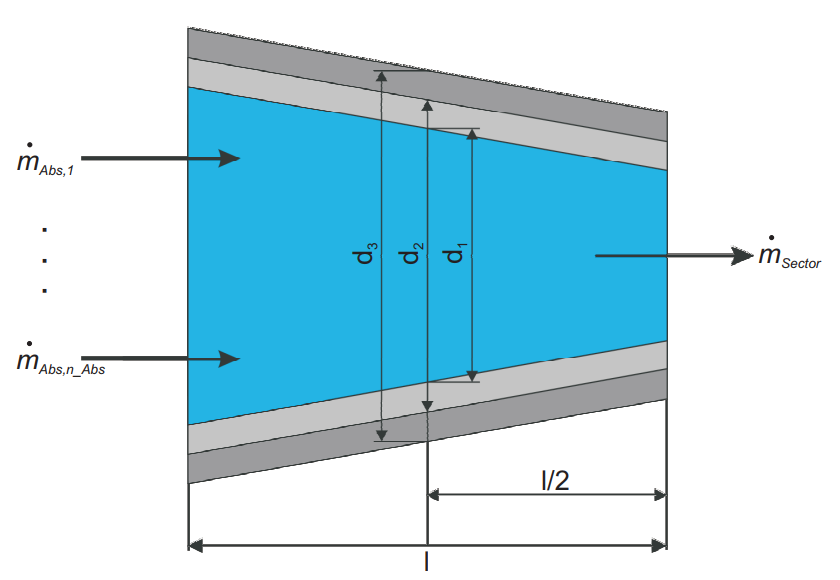
\includegraphics[width=0.6\textwidth]{fig/GeometrieHeader}}
    \caption[Geometrie des primären Headers]{Geometrie des primären Headers \cite[S.97]{DissGall}}
    \label{fig_header}
\end{figure}

\newpage
Schließlich ergibt sich der Enthalpiestrom am Receiveraustritt durch äquivalente Inbezugnahme des zweiten Headers.
Der Austrittsenthalpiestrom $\dot{H}_{\mathrm{out}}$ ergibt sich zu
\begin{equation} \label{eq_Headerout1}
\dot{H}_{\mathrm{out}} = \dot{H}_{\mathrm{sector,mixed}} + \QDotLoss{header,2},
\end{equation}
% \centerline{\small{\textsf{\textbf{Formel \ref{eq_Label}:}} Beschriftung}}
\myequations{\quad Entahlpiestrom am Receiveraustritt}

\vspace*{-\baselineskip}was identisch mit
\begin{equation} \label{eq_Headerout2}
h_{\mathrm{out}} = h_{\mathrm{sector,mixed}} + \frac{\QDotLoss{header,2}}{\MDotReceiver}
\end{equation}
% \centerline{\small{\textsf{\textbf{Formel \ref{eq_Label}:}} Beschriftung}}
\myequations{\quad Spezifische Entahlpie am Receiveraustritt}

\vspace*{-\baselineskip}ist.
Dabei ist $\MDotReceiver$ der Luftmassenstrom durch den gesamten Receiver, also der Summe der Luftmassenströme durch alle einzelnen Cups.
Der Wärmeverlust im sekundären Header wird analog zu Gleichung \ref{eq_VerlustwärmeHeader} mit $\QDotLoss{header,2}$ berücksichtigt und die Austrittstemperatur $T_{\mathrm{out}}$ ergibt sich erneut aus der Funktion $T(h)$.
Der Massenstrom des Gesamtreceivers ist messbar und dient dem System als Eingangsgröße. \cite[S.92]{DissGall}


\subsubsection*{Massenbilanzen} \label{subsubsec_Massenbilanzen}
Die Massenströme der Luft am Receivereintritt und -austritt werden als identisch angenommen, da keine Druckunterschiede in der Modellierung betrachtet werden.
Die Massenströme jedes einzelnen Absorbercups $\dot{m}_{\IndexAbsorber, i}$ können über den Gesamtmassenstrom $\MDotReceiver$ errechnet werden.
Da die Ventile an jedem Sektor als vollständig geöffnet betrachtet werden, sind die Absorbercupmassenströme lediglich von ihrem individuellen Blendendurchmesser im Rohrstück (vgl. \ref{subsec_GrundlagenAnnahmen}) abhängig.
Das Massenstromgesetz für eine Blende zeigt Gleichung \ref{eq_MassenstromgesetzBlende}:
\begin{equation} \label{eq_MassenstromgesetzBlende}
    \dot{V}=\alpha_0 A_0 \sqrt{\frac{2 \Delta p}{\rho}}
\end{equation}
% \centerline{\small{\textsf{\textbf{Formel \ref{eq_Label}:}} Beschriftung}}
\myequations{\quad Massenstromgesetz einer Blende}

Dies ist für Luft als Medium gleichbedeutend mit
\begin{equation} \label{eq_MassenstromBlende}
\dot{m} = \alpha_0 \frac{\pi \OrificeDiameter^2}{4} \sqrt{2 \rho_{\mathrm{air}} \Delta p },
\end{equation}
% \centerline{\small{\textsf{\textbf{Formel \ref{eq_Label}:}} Beschriftung}}
\myequations{\quad Berechnung des Massenstroms an einer Blende}

\vspace*{-\baselineskip}wobei $\alpha_0$ ein Durchflusskoeffizient ist, $\OrificeDiameter$ der Blendendurchmesser, $\rho_{\mathrm{air}}$ die Dichte der Luft und $\Delta p$ die Druckdifferenz vor und hinter der Blende.
Für die in dem System vorliegenden hohen Reynoldszahlen kann der Durchflusskoeffizient als konstant angesehen werden \cite{IdingSolarPaces}.
Weiterhin ist für konstante Massenströme auch die Druckdifferenz konstant und die Dichte der Luft aufgrund der Vernachlässigung von Druckänderungen im System ebenfalls.
Der Massenstrom ist daher direkt proportional zum Quadrat des Blendendurchmessers:
\begin{equation} \label{eq_AbhängigkeitMassenstrom}
    \dot{m} \propto \OrificeDiameter^2
\end{equation}
% \centerline{\small{\textsf{\textbf{Formel \ref{eq_Label}:}} Beschriftung}}
\myequations{\quad Zusammenhang zwischen Massenstrom und Blendendurchmesser}

Dementsprechend ergibt sich der Massenstrom eines einzelnen Cups durch die Eingangsgröße $\MDotReceiver$ und alle Blendendurchmesser im Receiver gemäß
\begin{equation} \label{eq_BerechnungMassenstrom}
    \dot{m}_{\IndexAbsorber, i} =\MDotReceiver \cdot \frac{\OrificeDiameter[,i]^2}{\sum_j^{n_{\mathrm{cups}}}\OrificeDiameter[,j]^2}
\end{equation}
% \centerline{\small{\textsf{\textbf{Formel \ref{eq_Label}:}} Beschriftung}}
\myequations{\quad Berechnung der Massenströme einzelner Absorbercups}


\section{Zielpunktregelung} \label{sec_Zielpunktregelung}
Neben der in Abschnitt \ref{subsec_Receiver} erwähnten Notwendigkeit der Zielpunktregelung zur Vermeidung zu hoher Temperaturen auf der Receiver Front, ist ein weiteres wesentliches Ziel, die Maximierung des wirtschaftlichen Ertrags des Kraftwerkes.
Nachfolgend wird das daraus resultierende Optimierungsproblem erläutert sowie einige Zielpunktregelungen aus der Literatur vorgestellt.
Im Anschluss wird eine Zielpunktstrategie mit Ventil-Analogie nach García \textit{et al.} \cite{Garcia2} detaillierter beschrieben.

\subsection{Optimierungsproblem der Zielpunktregelung} \label{subsec_OptimierungZielpunkte}
Eine optimale Ausrichtung der Heliostaten wird erreicht, wenn die Temperatur an jedem Cup des Receivers gleich der maximal zulässigen Temperatur ist, da der Receiver dann die meiste Leistung aufnimmt.
Aufgrund der Tatsache, dass ein Heliostat allerdings einen Brennfleck erzeugt, der mehrere Cups unterschiedlich beeinflusst, kann die Temperatur eines einzelnen Cups nicht durch einen Heliostaten angepasst werden, ohne die Temperatur der anderen Cups zu verändern.
Aus diesem Grund kann es unmöglich sein, die optimale Lösung zu finden, bei der an jedem Cup des Receivers die maximale Temperatur vorliegt.
Um die aufgenommene Leistung $P_{\mathrm{receiver}}$ zu maximieren, sollte also nicht die Temperatur jedes einzelnen Cups betrachtet werden, sondern die Leistung des Gesamtsystems unter Einhaltung der Grenztemperatur der Cups.
Das zugehörige Optimierungsproblem ergibt sich dann gemäß Gleichung \ref{eq_OptimierungZielpunkte}, wobei $T_{\mathrm{front,i}}$ die jeweilige Fronttemperatur des Cups $i$ und $(x_{h}, y_{h})$ die Zielpunktkoordinaten eines jeden Heliostaten $h$ darstellen.
Anstelle der maximalen Temperatur wird in der Literatur alternativ auch die maximale Flussdichte genutzt. \cite[S.15]{DissZanger}

\begin{equation} \label{eq_OptimierungZielpunkte}
    \begin{gathered}
\max \quad P_{\mathrm{receiver}}=f(T,x,y)  \qquad \\
        \begin{aligned}
T_{\mathrm{front,i}} \leq T_{\mathrm{front,max}}, \qquad                 & \forall~i \in \left\{1, ..., n_{\mathrm{cups}} \right\}       \\
\left(x_{h}, y_{h}\right) \in \mathbb{R}^2, \qquad & \forall~h \in \left\{1, ..., n_{\mathrm{heliostats}} \right\}
        \end{aligned}
    \end{gathered}
\end{equation}

\vspace*{-2.95\baselineskip}
\qquad subject to:
\vspace*{1.95\baselineskip}
\myequations{\quad Kontinuierliches Optimierungsproblem der Zielpunktregelung}
% \centerline{\small{\textsf{\textbf{Formel \ref{eq_OptimierungZielpunkte}:}} Kontinuierliches Optimierungsproblem der Zielpunktregelung}}

Die kontinuierliche Gleichung \ref{eq_OptimierungZielpunkte} erlaubt dem Heliostaten alle möglichen Zielpunkte in der Ebene $\mathbb{R}^2$.
Wie bereits in Kapitel \ref{subsec_Diskretisierung} erwähnt, geht die Diskretisierung eines Modells jedoch mit geringerem Rechenaufwand einher \cite[S.85]{DissBelhomme}.
Durch Definition einer Teilmenge möglicher diskreter Zielpunktkoordinaten $A$ wird eine mathematische Beschreibung des Problems wie in Gleichung \ref{eq_OptimierungZielpunkteDiskret} erreicht:

\begin{equation} \label{eq_OptimierungZielpunkteDiskret}
    \begin{gathered}
\max \quad P_{\mathrm{receiver}}=f(T,x,y)  \qquad \\
        \begin{aligned}
T_{\mathrm{front,i}} \leq T_{\mathrm{front,max}}, \qquad      & \forall~i \in \left\{1, ..., n_{\mathrm{cups}} \right\}       \\
\left(x_{h}, y_{h}\right) \in A, \qquad & \forall~h \in \left\{1, ..., n_{\mathrm{heliostats}} \right\}
        \end{aligned}
    \end{gathered}
\end{equation}

\vspace*{-2.95\baselineskip}
\qquad subject to:
\vspace*{1.95\baselineskip}
\myequations{\quad Diskretes Optimierungsproblem der Zielpunktregelung}
% \centerline{\small{\textsf{\textbf{Formel \ref{eq_OptimierungZielpunkteDiskret}:}} Diskretes Optimierungsproblem der Zielpunktregelung}}

Um eine möglichst hohe Leistung zu absorbieren, werden die Heliostaten bevorzugt auf die Mitte gerichtet, sodass alle Brennflecke vollständig auf dem Receiver abgebildet werden und die Streuungsverluste (vgl. Abschnitt \ref{subsubsec_Streuung}) so gering wie mögich sind.
Werden jedoch alle Heliostaten auf die Mitte ausgerichtet, wird die zulässige Fronttemperatur des Receivers überschritten.
Aus diesem Grund werden einige Heliostaten bei klarem Himmel defokussiert.
Obwohl alle Heliostaten, unabhängig von ihrer Entfernung zum Receiver, eine ähnliche Leistung reflektieren, ist der Einfluss receivernaher Heliostaten auf einzelne Cups aufgrund des kleineren Brennfleckes größer.
Daher werden diese Heliostaten vorzugsweise zur Defokussierung verwendet, um die physikalischen Limitierungen des Receivers auch bei starker solarer Einstrahlung einzuhalten.

Es ist zu beachten, dass eine optimale Lösung des in Gleichung \ref{eq_OptimierungZielpunkteDiskret} formulierten Problems nicht notwendigerweise die optimale Lösung in Bezug auf das reale System ist, da Modellfehler auftreten und das reale System Störungen unterworfen ist.
Sie verändern die Flussdichteverteilungen der Heliostaten und können daher die abgefangene Leistung einzelner Cups verringern oder auch erhöhen.
Durch den Nachführfehler (Kapitel \ref{subsubsec_Nachführfehler}) beispielsweise könnte die erlaubte Temperatur des Receivers überschritten werden, wenn die Verschiebung hin zu einem bereits kritisch heißen Cup geschieht. \cite[S.16]{DissZanger}

Wolken widerum reduzieren die reflektierte Strahlung während ihres Durchzuges, was die Möglichkeit bietet, die Zielpunkte stäker zu fokussieren.
Zieht die Wolke weiter, während die Heliostaten immer noch überwiegend in Richtung Receiver-Zentrum fokussieren, kann dies zu einer Überschreitung der maximalen Temperatur oder Temperaturgradienten führen.
Diesen Umstand zeigt die Abbildung \ref{fig_EinflussWolke} qualitativ.
Hier wird ein konstanter Luftmassenstrom im Inneren des Receivers vorausgesetzt, sodass die Temperatur auf der Vorderseite des Receivers ($T_{\mathrm{abs}}$) und die Luftaustrittstemperatur im Receiver $T_{\mathrm{outlet}}$ lediglich von der solaren Einstrahlung $P_{\mathrm{solar}}$ abhängig ist.

Es ist erkennbar, dass die solare Einstrahlung durch eine Wolke ab dem Zeitpunkt $t_1$ abnimmt und sich ein Gleichgewichtszustand mit geringerer Leistung einstellt.
Zum Zeitpunkt $t_2$ werden auch die Heliostaten mit geringer Entfernung zum Receiver stärker fokussiert und die aufgenommene Leistung sowie die Receiver- und Lufttemperatur steigen an.
Aufgrund der geringeren Einstrahlung durch die Wolke kann $P_{\mathrm{solar}}$ nicht das identische Niveau wie vor Beginn des Wolkeneinflusses erreichen, durch die Fokussierung wird jedoch ein Teil des Verlustes ausgeglichen.
Aus diesem Grund besteht allerdings die Gefahr, dass zu dem Zeitpunkt $t_3$, an dem die Wolke keinen Einfluss mehr hat, die notwendige Defokussierung der Heliostaten nicht abgeschlossen ist.
In der Folge ist mit einer Überschreitung der Grenztemperaturen und der Temperaturgradienten zu rechnen.

\begin{figure}[h!]
    \centering
    \setlength{\fboxsep}{1pt}
    \setlength{\fboxrule}{1pt}
    \fbox{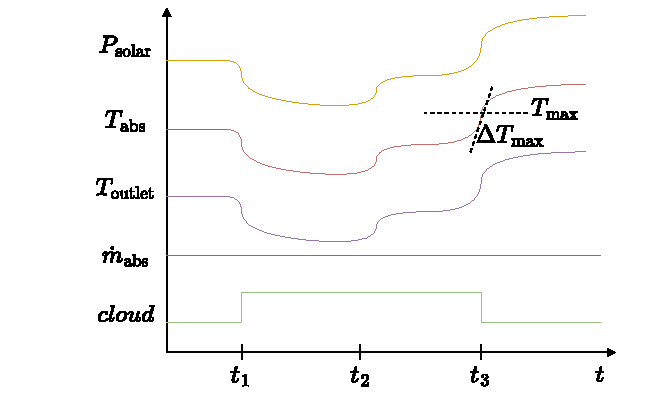
\includegraphics[width=0.65\textwidth]{fig/CloudVerlauf}}
    \caption[Darstellung der potenziellen Gefahr einer durchziehenden Wolke]{Darstellung der potenziellen Gefahr einer durchziehenden Wolke}
    \label{fig_EinflussWolke}
\end{figure}

\subsection{Existierende Algorithmen} \label{subsec_ZielpunktregelungLiteratur}
Eine Übersicht über verschiedene Algorithmen zur Zielpunktregelung wurde von Oberkirsch in \cite{DissOberkirsch} aufgestellt.
An dieser Stelle werden beispielhaft einige dieser Regelungen kurz vorgestellt, bevor in Absatz \ref{subsec_ZielpunktregelungGarcia} eine Zielpunktregelung nach García detaillierter erklärt wird.

Maldonado \textit{et al.} \cite{Maldonado}\cite{Maldonado2} entwickelte beispielsweise einen iterativen Algorithmus namens \textit{Local Search}.
Dieser beginnt bei einer initialen Lösung zur Zielpunktverteilung und untersucht für jede Iteration, ob eine Verschiebung zu diskreten benachbarten Zielpunkten im Hinblick auf die Gesamtleistung des Receivers einen Vorteil bringt.
Der jeweilige Heliostat ändert seine Ausrichtung dann so, dass die Leistung maximal gesteigert wird, sofern eine Steigerung möglich ist.
Auf diese Weise wird nach und nach über jeden benachbarten Zielpunkt und über alle Heliostaten iteriert.

In einer Arbeit von Cruz \textit{et al.} \cite{Cruz} wird ein Algorithmus zur Zielpunktsteuerung vorgeschlagen, der eine gewünschte Flussdichteverteilung auf dem Receiver erreichen soll.
Das Problem wird durch eine zweistufige Optimierung gelöst; die erste Stufe bestimmt mittels eines meta-heuristischen Algorithmus die zu optimierenden Heliostaten und die zweite Stufe legt mit einem gradientenbasierten Suchverfahren die Zielpunkte dieser Heliostaten fest. Erfolgreiche Tests dieses Verfahrens werden in der Veröffentlichung jedoch nur mit 50 aktiven Heliostaten beschrieben.

Vant-Hull \textit{et al.} \cite{VantHull2}\cite{VantHull3} hat unter anderem das \textit{Dynamic Aimpoint Processing System} (\textit{DAPS}) entwickelt; eine Regelung die im Wesentlichen das Überschreiten maximaler Flussdichten verhindern soll.
Dazu wird der Teil des Receivers mit der höchsten überschrittenen Flussdichte gemessen oder simulativ bestimmt und anschließend identifiziert, welcher Heliostat den größten Einfluss auf diesen Cup hat; dieser Heliostat wird anschließend defokussiert.
In einem iterativen Prozess wird dieses Verfahren wiederholt, bis die Flussdichte an keinem Cup mehr überschritten wird.

García \textit{et al.} \cite{Garcia1} stellte einen Algorithmus vor, der das Problem nicht als MIMO System definiert, also mit allen Heliostaten als Eingangsgrößen und allen Zielpunkten als separat zu berechnende Ausgangsgrößen, sondern als System aus 6 \textit{SISO} (\textbf{S}ingle \textbf{I}nput \textbf{S}ingle \textbf{O}utput) Subsystemen.
Dazu werden die Heliostaten je nach Entfernung zum Receiver in drei Gruppen eingeteilt.
Für jede Gruppe werden dann zwei Faktoren eingeführt: Ein Faktor, der das \textit{shifting}, also die Verschiebung der Zielpunktmitte jeder Gruppe vom Zentrum her beschreibt und einer, der die \textit{dispersion}, also die Streuung der Heliostaten von dieser Gruppenmitte aus angibt.
Auf diese Weise werden sechs Subsysteme gebildet, die von separaten \textit{PID}-Reglern geregelt werden.


\subsection{Zielpunktstrategie mit Ventil-Analogie nach García} \label{subsec_ZielpunktregelungGarcia}
Detailliert wird ein Algorithmus zur Zielpunktverteilung vorgestellt, welcher ebenfalls von García \textit{et al.} \cite{Garcia2} veröffentlicht wurde und mit Gruppierung von Heliostaten und \textit{dispersion} (vgl. Kapitel \ref{subsec_ZielpunktregelungLiteratur}) der Heliostaten arbeitet.
Er wird in Kombination mit einer modellprädiktiven Regelung eines zylindrischen Receivers vorgestellt, der eine maximal erlaubte Flussdichte als physikalische Limitierung vorgibt.
Der Algorithmus an sich kann jedoch auch in Kombination mit dem Modell eines rechteckigen Receivers und der Temperatur als Limitierung verwendet werden.
Für diese Arbeit ist die vorgestellte Regelung nicht relevant, an dieser Stelle wird demnach lediglich die Zielpunktstrategie vorgestellt.
Von besonderer Relevanz ist dabei einerseits die Gruppierung der Heliostaten und andererseits das Verhalten der einzelnen Heliostaten innerhalb der Gruppen in Abhängigkeit der von García eingeführten Stellgrößen.

\subsubsection*{Gruppierung der Heliostaten} \label{subsubsec_Gruppierung}
Da in \cite{Garcia2} ein Rundum-Heliostatenfeld (vgl. Abschnitt \ref{subsec_Heliostaten}) untersucht wird, erfolgt zunächst eine Einteilung der Heliostaten in 18 Gruppen, die auf jeweils eins der 18 rechteckigen Teilstücke des insgesamt zylindrisch aufgebauten Receivers gerichtet werden.
Anschließend wird jede dieser Gruppen noch dreifach unterteilt.
Einerseits entstehen zwei Gruppen mit einem Radius von $<\SI{400}{\metre}$ Entfernung zum Receiver, welche im gleichen Teil des Feldes stehen und eine ähnliche Leistung zum Receiver reflektieren können.
Die dritte Gruppe umfasst alle weiteren Heliostaten mit größerem Abstand zum Receiver. \cite[S.8-10]{Garcia2}\\
Abbildung \ref{fig_VerteilungHeliostateGarcia} zeigt diese Einteilung in $18 \times 3$ Gruppen von Heliostaten; die Gruppen sind farblich in Rot, Grün und Blau dargestellt.

\begin{figure}[h!]
    \centering
    \setlength{\fboxsep}{1pt}
    \setlength{\fboxrule}{1pt}
\fbox{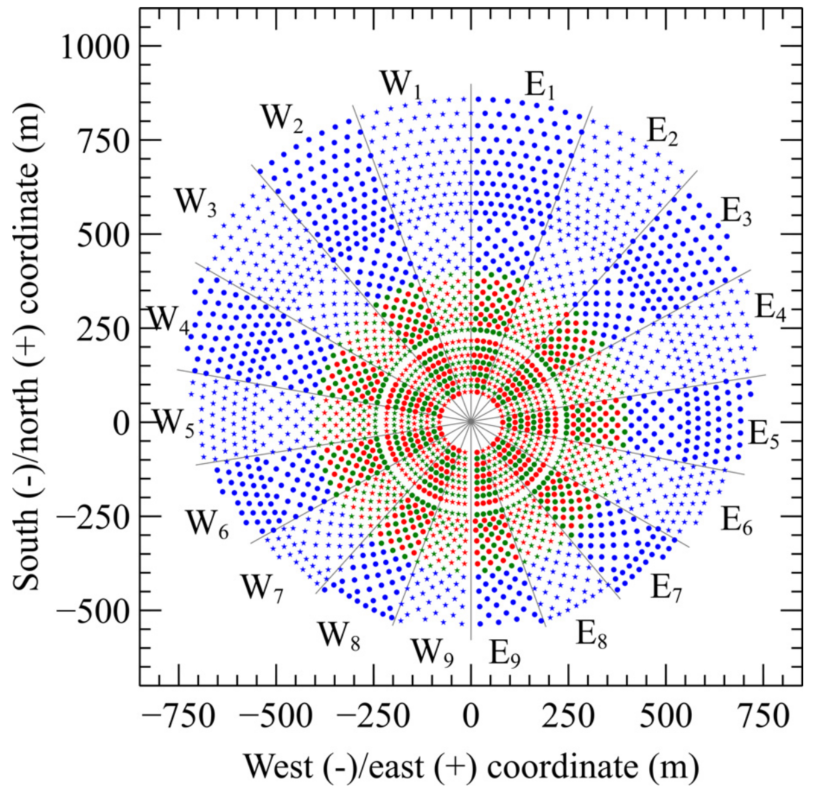
\includegraphics[width=0.53\textwidth]{fig/GarciaFeld}}
    \caption[Einteilung des Heliostatenfeldes des Gemasolar-Kraftwerkes in Sevilla in 54 Gruppen]{Einteilung des Heliostatenfeldes des Gemasolar-Kraftwerkes in Sevilla in 54 Gruppen \cite[S.10]{Garcia2}}
    \label{fig_VerteilungHeliostateGarcia}
\end{figure}

\subsubsection*{Verhalten der Heliostaten innerhalb einer Gruppe} \label{subsubsec_Gruppenverhalten}
Das von García vorgestellte Verfahren besitzt zwei Parameter pro Gruppe, um das Verhalten der einzelnen Heliostaten innerhalb jeder Gruppe zu beeinflussen.
Einerseits den \textit{dispersion factor} $\kappa$, der Auskunft über die Streuung der Heliostaten innerhalb der Gruppe gibt und andererseits den Parameter $y_{\mathrm{Cent}}$, der die vertikale Position des \gans{Schwerpunktes} aller Zielpunkte auf dem Receiver beeinflussen kann \cite[S.5]{Garcia2}.
Die Ventil-Analogie bezieht sich auf den Faktor $\kappa$, ein kleiner Wert führt zu einer hohen Flussdichtekonzentration (geöffnetes Ventil) und ein großer Wert zu einer geringeren Konzentration der Flussdichte (geschlossenes Ventil).
Der zweite Parameter ist bei zylindrischen Receivern notwendig, kann aber nachfolgend vernachlässigt werden und wird zu $y_{\mathrm{Cent}} = 0$ gesetzt.
Da sowohl nachfolgend als auch in der Arbeit von García $x_{\mathrm{Cent}} = 0$ gilt, wird sichergestellt, dass der Schwerpunkt aller Gruppen im Zentrum des Receivers bei $(0,0)$ liegt.
Abbildung \ref{fig_DispersionVeranschaulichung} zeigt den Einfluss der beiden Stellgrößen exemplarisch, wobei erkennbar ist, dass der Faktor $\kappa_1 > \kappa_2$ sein muss, da die Entfernung der Zielpunkte untereinander größer ist.

\enlargethispage{\baselineskip}
\begin{figure}[h!]
    \centering
    \setlength{\fboxsep}{1pt}
    \setlength{\fboxrule}{1pt}
\fbox{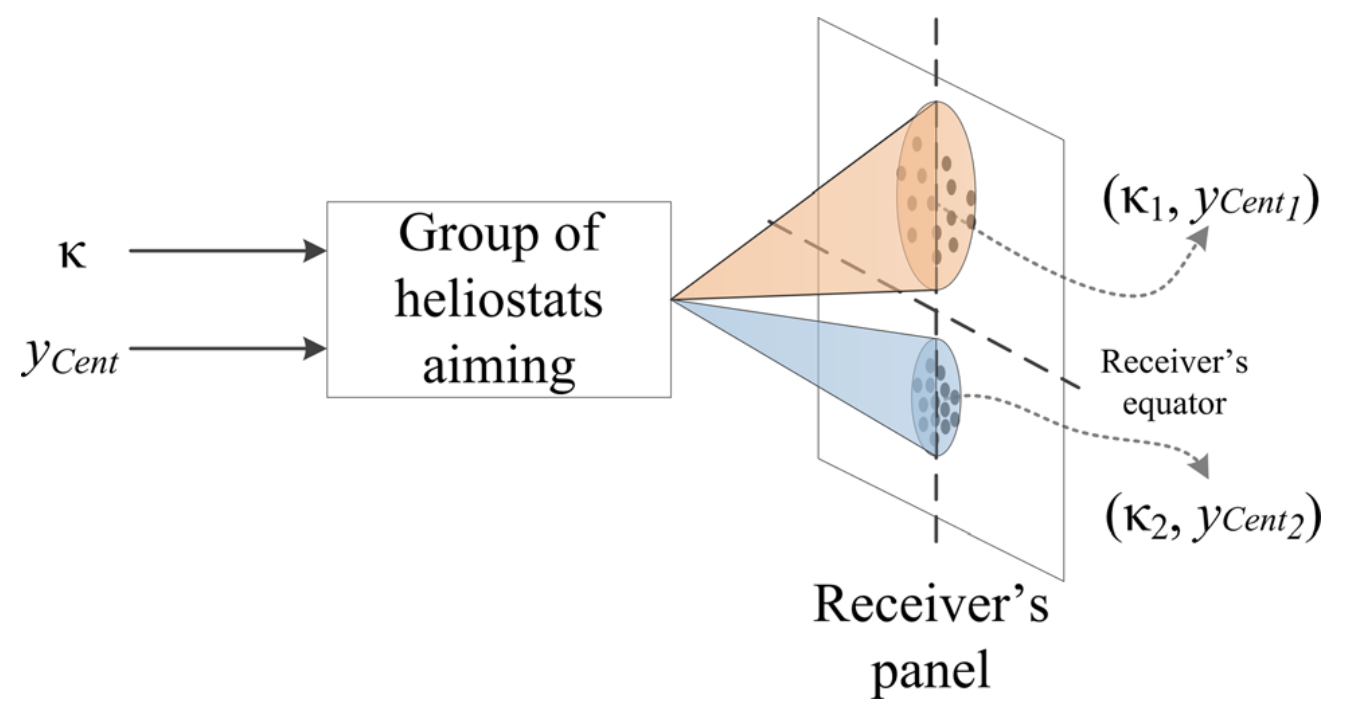
\includegraphics[width=0.58\textwidth]{fig/GarciaDispersionSymbolisch}}
\caption[Veranschaulichung der Stellgrößen des gewählten Algorithmus]{Veranschaulichung der Stellgrößen des gewählten Algorithmus \cite[S.7]{Garcia2}}
    \label{fig_DispersionVeranschaulichung}
\end{figure}

Die Zielpunkte der Gruppe erfüllen zwei Kriterien, wenn sich durch die Stellgrößen $\kappa$ und $y_{\mathrm{Cent}}$ ein Gleichgewichtszustand eingestellt hat:
\begin{itemize}
\item[1.] Jeder einzelne Punkt wird so nah wie möglich am festgelegten Schwerpunkt der Gruppe sein und dabei einen individuellen Minimalabstand zum nächsten Zielpunkt $r$, welcher von $\kappa$ abhängt, nicht unterschreiten.
\item[2.] Ihr Gruppenschwerpunkt wird mit dem durch $(x_{\mathrm{Cent}}, y_{\mathrm{Cent}})$ vorgegebenen Punkt, hier also $(0,0)$, übereinstimmen.
\end{itemize}

\textit{Kriterium 1:}\\
Ein statischer Parameter $a$ wird verwendet, um die Heliostaten einer Gruppe zu organisieren.
Dieser Parameter weist jedem Heliostaten individuell einen Wert $\alpha$ zu, welcher sich aus der Anzahl der Heliostaten $n$ und $a$ ergibt (siehe Gleichung \ref{eq_GarciaAlpha} und \ref{eq_GarciaDeltaAlpha}).

\begin{gather}
    \alpha \in \left[-a, -a+\Delta\alpha, -a+2\Delta\alpha,..., a\right] \label{eq_GarciaAlpha}\\
    \text{\myequations{\quad Berechnung des individuellen Heliostatenparameters $\alpha$}}
\text{Mit:\qquad}\Delta\alpha = \frac{2a}{n-1}, \quad \forall~\left\{n \in \mathbb{N}, n > 1 \right\} \qquad\qquad \label{eq_GarciaDeltaAlpha}
\end{gather}
% \centerline{\small{\textsf{\textbf{Formel \ref{eq_GarciaAlpha} und \ref{eq_GarciaDeltaAlpha}:}} Berechnung des individuellen Heliostatenparameters $\alpha$}}
\myequations{\quad Berechnung von $\Delta\alpha$}

Daraus kann für jeden Heliostaten der Radius $r$ berechnet werden, der den Mindestabstand zu benachbarten Zielpunkten vorgibt und damit das zentrale Element der Zielpunktstrategie ist.
Er ergibt sich gemäß \ref{eq_GarciaMindestabstand}, wobei $\kappa$ wie beschrieben die Stellgröße des Reglers zur Zielpunktstreuung darstellt und $\beta$ ein Skalierungsfaktor ist.

\begin{equation} \label{eq_GarciaMindestabstand}
    r=\frac{\kappa}{1+\left|\frac{\alpha}{\kappa}\right|^{2\kappa}}\cdot\beta
\end{equation}
% \begin{center}
%     \begin{varwidth}{0.95\textwidth}
% \small{\textsf{\textbf{Formel \ref{eq_GarciaMindestabstand}:}} Bestimmung des Mindestabstandes eines jeden Zielpunktes zum nächstgelegenen Zielpunkt der Heliostatengruppe}
%     \end{varwidth}
% \end{center}
\myequations{\quad Bestimmung des Mindestabstandes eines jeden Zielpunktes zum nächstgelegenen\\\hspace*{0.3cm} Zielpunkt der Heliostatengruppe}

Abbildung \ref{fig_Verteilunglpha} zeigt die sich ergebenden Radien je nach individuellem $\alpha$-Wert exemplarisch für $\kappa=2$ bzw. $\kappa=5$.
Es ist erkennbar, dass die Wahl hoher Werte für $a$ kleine Abstände zwischen den Zielpunkten zur Folge haben wird.

\begin{figure}[h!]
    \centering
    \setlength{\fboxsep}{1pt}
    \setlength{\fboxrule}{1pt}
    \fbox{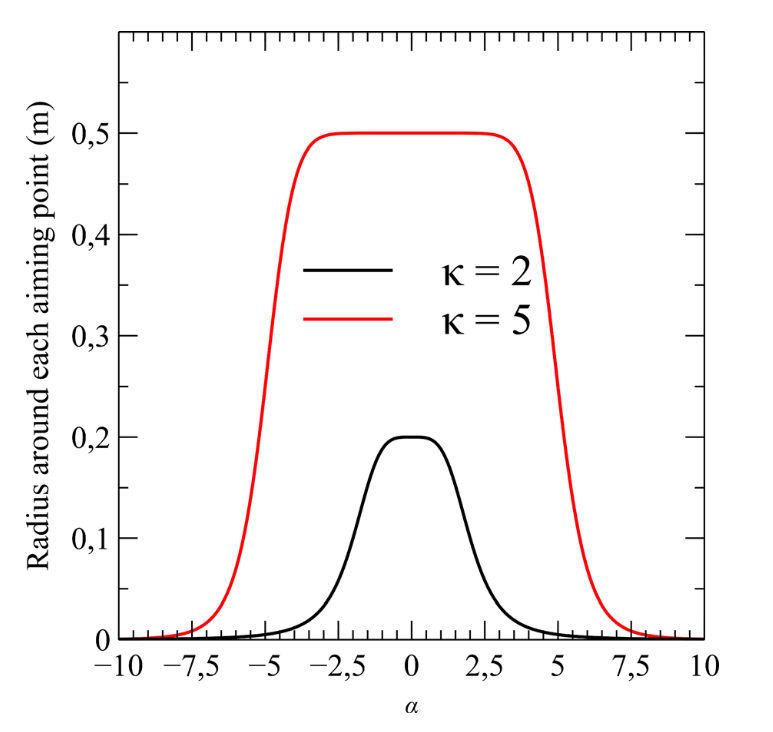
\includegraphics[width=0.5\textwidth]{fig/GarciaVerteilungAlpha.png}}
    \caption[Minimalabstände der Zielpunkte je $\alpha$-Wert]{Minimalabstände der Zielpunkte je $\alpha$-Wert \cite[S.9]{Garcia2}}
    \label{fig_Verteilunglpha}
\end{figure}

Auf den durch $\kappa$ festgelegten Mindestabständen aufbauend, ergeben sich, sofern noch kein Gleichgewichtszustand erreicht ist, Bewegungen der Heliostaten und Zielpunkte.
Die Distanz, die zwischen zwei Zielpunkten zurückgelegt werden muss, ist mit $\Delta D$ benannt und setzt sich aus $\Delta x$ und $\Delta y$ zusammen.
Diese bezeichnen Strecken in beiden Dimensionen, die auf dem Receiver zwischen zwei Zielpunkten zurückgelegt werden müssen.
In Abbildung \ref{fig_AbständeGarcia} ist für eine Gruppe aus fünf Heliostaten dargestellt, welche Zeilpunktabstände dabei alle relevant sind.
Exemplarisch ist die notwendige Evaluation der Radien $r_1$ und $r_2$ sowie der zugehörigen Distanz $d_{1-2}$ dargestellt.

\newpage
\begin{figure}[h!]
    \centering
    \setlength{\fboxsep}{1pt}
    \setlength{\fboxrule}{1pt}
    \fbox{\includegraphics[width=0.5\textwidth]{fig/AbständeGarcia.png}}
    \caption[Visualisierung der relevanten Distanzen zwischen Zielpunkten für eine Gruppe aus fünf Heliostaten nach García]{Visualisierung der relevanten Distanzen zwischen Zielpunkten für eine Gruppe aus fünf Heliostaten nach García \cite[S.7]{Garcia2}}
    \label{fig_AbständeGarcia}
\end{figure}


Um sicherzustellen, dass der Abstand eines jeden Zielpunktes zu allen anderen Zielpunkten der Gruppe eingehalten wird, wiederholen sich diese Berechnungsvorschriften für jedes mögliche Pärchen aus Heliostaten \cite[S.9]{Garcia2}.
Anschließend wird der Durchschnitt der berechneten Distanzen eines Zielpunktes relativ zu den anderen Heliostaten ($\overline{\Delta x_{\mathrm{TP_n}}}$) und ($\overline{\Delta y_{\mathrm{TP_n}}}$) errechnet \cite[S.10]{Garcia2}.

\newpage
\textit{Kriterium 2:}\\
Wie erläutert, kommt es nun also zu erforderlichen Bewegungen der Zielpunkte auf dem Receiver.
Diese Bewegungen müssen nun so reguliert werden, dass der Schwerpunkt der Heliostatengruppe weiterhin mit dem vorgegebenen Gruppenmittelpunkt übereinstimmt.
Dazu wird $\Delta D_{\mathrm{Centroid}}$ bestimmt, ein Wert, der angibt, wie weit sich das Gruppenschwerpunkt $(x_{\mathrm{Actual Centroid}}, y_{\mathrm{Actual Centroid}})$ vom geforderten Punkt $(x_{\mathrm{Cent}}, y_{\mathrm{Cent}})$ unterscheidet.
Er berechnet sich nach Gleichung \ref{eq_GarciaGruppenzentrumbewegung}, wobei $k_2$ eine Konstante zur Berücksichtigung der zulässigen Stellgeschwindigkeiten der Heliostaten darstellt. \cite[S.10]{Garcia2}

\begin{equation} \label{eq_GarciaGruppenzentrumbewegung}
\Delta D_{\mathrm{Centroid}} = k_2 \cdot \sqrt{\left(x_{\mathrm{Cent}}-x_{\mathrm{Actual Centroid}}\right)^2+\left(y_{\mathrm{Cent}}-y_{\mathrm{Actual Centroid}}\right)^2}
\end{equation}
% \centerline{\small{\textsf{\textbf{Formel \ref{eq_GarciaGruppenzentrumbewegung}:}} Erforderliche Schwerpunktverschiebung der Zielpunktgruppe}}
\myequations{\quad Erforderliche Schwerpunktverschiebung der Zielpunktgruppe}

Darauf aufbauend ergeben sich mathematisch erneut die erforderlichen Verschiebungen der Gruppe $\Delta X_{\mathrm{Group}}$ und $\Delta Y_{\mathrm{Group}}$ \cite[S.10]{Garcia2}.
Zuletzt können die tatsächlichen Koordinaten eines jeden Zielpunktes im nächsten Zeitschritt durch Verschiebung der vorigen Koordinaten um $\overline{\Delta x,y_{\mathrm{TP_n}}}$ und $\overline{\Delta X,Y_{\mathrm{Group}}}$ nach Gleichung \ref{eq_VerschiebungZielpunkteGarcia} bestimmt werden.
Die vollständige Darstellung des hier vorgestellten Algorithmus nach García \textit{et al.} \cite{Garcia2} zeigt Abbildung \ref{fig_GarciaAlg}.

\begin{equation} \label{eq_VerschiebungZielpunkteGarcia}
    \begin{gathered}
        x_{\mathrm{TP_n}} = x^{\mathrm{Previous}}_{\mathrm{TP_n}} + \overline{\Delta x_{\mathrm{TP_n}}} + \overline{\Delta X_{\mathrm{Group}}} \\
        y_{\mathrm{TP_n}} = y^{\mathrm{Previous}}_{\mathrm{TP_n}} + \overline{\Delta y_{\mathrm{TP_n}}} + \overline{\Delta Y_{\mathrm{Group}}}
    \end{gathered}
\end{equation}
% \centerline{\small{\textsf{\textbf{Formel \ref{eq_Label}:}} Beschriftung}}
\myequations{\quad Verschiebung der Zielpunkte durch Zielpunktstrategie nach García}


\begin{figure}[p]
    \centering
\setlength{\fboxsep}{3pt}
    \setlength{\fboxrule}{1pt}
    \fbox{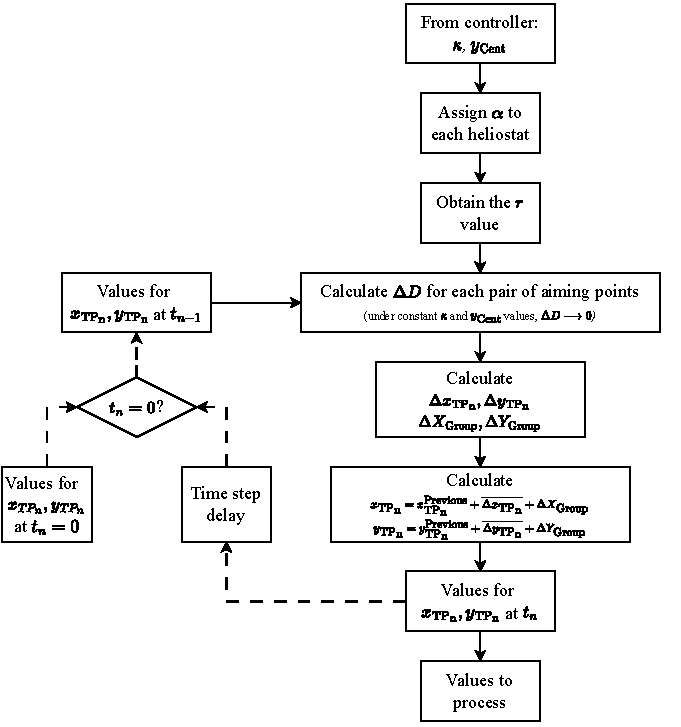
\includegraphics[width=0.9\textwidth]{fig/AlgorithmusGarcia.pdf}}
    \caption[Übersicht der vollständigen Zielpunktstrategie nach García]{Übersicht der vollständigen Zielpunktstrategie nach García \cite[S.10]{Garcia2}}
    \label{fig_GarciaAlg}
\end{figure}

Eine beispielhafte Zielpunktverteilung für einen zunehmenden Faktor $\kappa$ und einem Gruppenzentrum in der Mitte des Receivers ist in Abbildung \ref{fig_GarciaZielpunkte} erkennbar.
Es wird deutlich, dass das Gruppenzentrum nach wie vor in der Mitte liegt und die Abstände zwischen den Zielpunkten dennoch sichtbar zunehmen.
Aufgrund des individuellen Parameters $\alpha$ sind die erforderlichen Mindestabstände jedoch nicht für alle Zielpunkte gleich groß.

\begin{figure}[h!]
    \centering
    \setlength{\fboxsep}{1pt}
    \setlength{\fboxrule}{1pt}
    \fbox{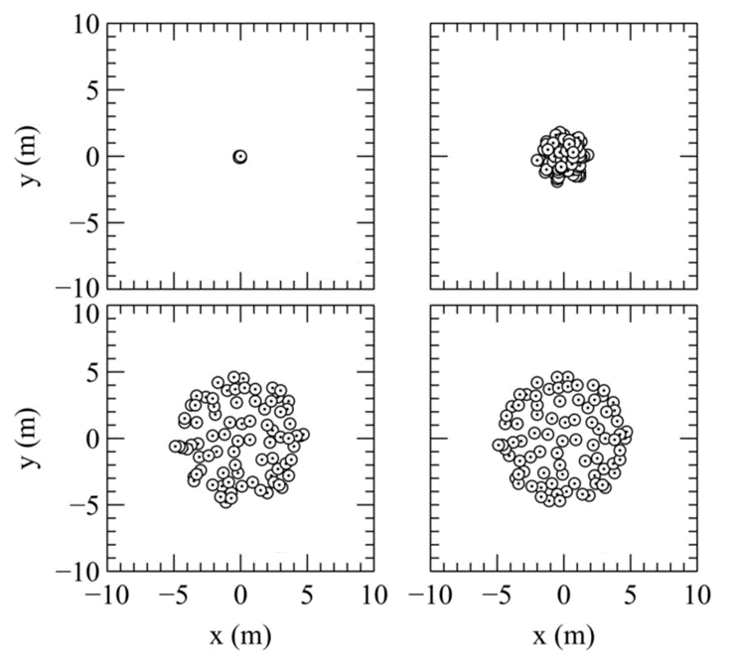
\includegraphics[width=0.75\textwidth]{fig/GarciaZielpunktewotime}}
    \caption[Beispielhafte Zielpunktverteilungen für einen zunehmenden $\kappa$ Wert]{Beispielhafte Zielpunktverteilungen für einen zunehmenden $\kappa$ Wert (nach \mbox{\cite[S.11]{Garcia2}})}
    \label{fig_GarciaZielpunkte}
\end{figure}

\subsubsection*{Zusammenfassung} \label{subsubsec_Zusammenfassung}
Letztlich handelt es sich bei dem vorgestellten Algorithmus von García um eine Strategie, um viele Heliostaten mit einer geringen Anzahl an Stellgrößen auf individuellen Bahnen zu bewegen.
Dafür werden pro Gruppe lediglich zwei Stellgrößen eingeführt, von der für rechteckige Receiver nur eine, der \textit{dispersion factor} $\kappa$, weiter betrachtet wird.
Dieser streut die Zielpunkte so, dass die Konzentration der Flussdichte wie durch ein Ventil geregelt wird.
Ein wesentlicher Vorteil des gewählten Algorithmus ist die enorme Reduzierung der Stellgrößen; statt die vorhandenen 2153 Heliostaten am Standort Jülich einzeln positionieren zu müssen, geschieht dies durch lediglich drei Stellgrößen.
Außerdem stehen als Endergebnis der Berechnung die einzelnen Zielpunkte der Heliostaten zur Verfügung.
Dies sorgt für eine gute Kompatibilität in der Modellbildung des gesamten Systems, wie es in Kapitel \ref{ch_Modellbildung} erläutert wird.


\section{Relevante Software} \label{sec_HardSoftware}
Die Modellbildung und die Simulationen in den nachfolgenden Kapiteln werden mithilfe der Programmiersprache \textit{Python} umgesetzt.
Dabei handelt es sich Stand März 2023 um die populärste Programmiersprache weltweit \cite{Statista}.
Nicht zuletzt aufgrund der Echtzeitfähigkeit und einfachen Syntax \cite[S.9]{Python} hat sie sich besonders im Bereich des \textit{machine learning} als Stand der Technik etabliert.
Darüber hinaus zeichnet sich Python durch ihre große Anzahl an professionellen Frameworks und Bibliotheken aus, welche es Entwicklern ermöglichen, auch komplexe Probleme mit geringem Aufwand zu lösen \cite[S.3]{Python}.
Zwei Beispiele für solche Frameworks, die auch in dieser Arbeit Verwendung finden, sind \gans{CasADi} und \gans{do-mpc}.

CasADi ist eine Open-Source Bibliothek für MATLAB/Octave, C++ und Python.
Sie dient der gradientenbasierten numerischen Optimierung mit einem besonderen Fokus auf der Regelungstechnik.
Durch CasADi soll besonders die symbolische Formulierung von gewöhnlichen Differentialgleichungen (ODEs) und differential-algebraischen Gleichungen (DAEs) erleichtert und damit die Formulierung und Lösung nicht-linearer Programme und Regelungsprobleme ermöglicht werden. \cite{Casadi}

\enlargethispage{\baselineskip}
Do-mpc ist ebenfalls eine Open-Source Bibliothek.
Sie basiert auf CasADi und ermöglicht die einfache Integration modellprädiktiver Regelungen und Zustandsvorhersagen mittels \textit{moving horizon estimation} (MHE).
Ihre Module vereinen \mbox{Simulations-,} Vorhersage- und Regelungskomponenten aus diesem Bereich \cite{Dompc2}.
